\documentclass[format=acmsmall, printccs]{acmart}
%\documentclass[sigconf]{acmart}

%%% Some recommended packages.
%\usepackage{booktabs}   %% For formal tables:
%                        %% http://ctan.org/pkg/booktabs
%\usepackage{subcaption} %% For complex figures with subfigures/subcaptions
%                        %% http://ctan.org/pkg/subcaption
\newif\iffull
\fullfalse

\usepackage{mathptmx}
\usepackage{graphicx}
\usepackage{mathtools}
\usepackage{amsmath}
\usepackage[utf8]{inputenc}
\usepackage{cleveref}
\usepackage{listings}
\usepackage{array}
\usepackage{breqn}
\usepackage{tikz}
\usepackage{algorithmicx}
\usepackage[Algorithm,ruled]{algorithm}
\usepackage{algpseudocode}
\usepackage{pifont,xspace}
\usetikzlibrary{automata,positioning,shapes.geometric}
\newcommand{\name}{{\sc Zeppelin}\xspace}
\newcommand{\Name}{\name}
\newcommand{\genesis}{Genesis\xspace}
\newcommand{\pushcode}[1][1]{\hskip\dimexpr#1\algorithmicindent\relax}
\newcolumntype{P}[1]{>{\centering\arraybackslash}p{#1}}

\usetikzlibrary{calc}
\usetikzlibrary{arrows}
\usetikzlibrary{decorations.markings}

\newcommand*{\StrikeThruDistance}{0.2cm}%
\newcommand*{\StrikeThru}{\StrikeThruDistance,\StrikeThruDistance}%


\tikzset{strike thru arrow/.style={
		decoration={markings, mark=at position 0.5 with {
				\draw [black, thick,-] 
				++ (-\StrikeThruDistance,-\StrikeThruDistance) 
				-- ( \StrikeThruDistance, \StrikeThruDistance);}
		},
		postaction={decorate},
	}}
	

\usepackage{times}
\usepackage[font=small]{caption}
%\usepackage{subcaption}
\usepackage{enumitem}
%\usepackage{usenix}
\usepackage{epsfig}
%\usepackage[TABBOTCAP]{subfigure}
\usepackage{color}
%\usepackage{thumbpdf}
\usepackage{verbatim}
%\usepackage{hyperref}
\usepackage{url}
%\usepackage{booktabs}
\usepackage{colortbl}
\usepackage{enumitem}
\usepackage[export]{adjustbox}
\usepackage{subfig}
\usepackage{mathtools}
\usepackage{amssymb}
\usepackage{amsthm}
\usepackage{multirow}% http://ctan.org/pkg/multirow
\usepackage{multicol}
\usepackage{hhline}
\usepackage{wrapfig}
\usepackage{array,ragged2e}
\newcommand{\minisection}[1]{\smallskip\noindent{\bf #1.}}
\newcommand{\secref}[1]{{\S\ref{#1}}}
\newcommand{\secsref}[2]{{Sections~\ref{#1} and \S\ref{#2}}}
\newcommand{\figref}[1]{{Figure~\ref{#1}}}
\newcommand{\figsref}[2]{{Figure~\ref{#1} and \ref{#2}}}
\newcommand{\appref}[1]{{Appendix~\ref{#1}}}
\newcommand{\thmref}[1]{{Theorem~\ref{#1}}}
\newcommand{\lemref}[1]{{Lemma~\ref{#1}}}
\newcommand{\corref}[1]{{Corollary~\ref{#1}}}
\newcommand{\proref}[1]{{Property~\ref{#1}}}
\newcommand{\tabref}[1]{{Table~\ref{#1}}}


\newcommand{\compactcaption}[1]{\vspace{-1em}\caption{#1}\vspace{-1em}}
\newcommand{\botcompactcaption}[1]{\caption{#1}\vspace{-1em}}
\newcommand{\topcompactcaption}[1]{\vspace{-1em}\caption{#1}\vspace{-0.5em}}

\newenvironment{compactitemize}
{
   \begin{itemize}[leftmargin=1.5em]
   \vspace{-1ex}
   \setlength{\topsep}{0pt}
   \setlength{\itemsep}{0em}
   \setlength{\parskip}{0pt}
   \setlength{\parsep}{0pt}
}
{
   \vspace{-1ex}
   \end{itemize}
}
\newenvironment{compact2itemize}
{
	\begin{itemize}[leftmargin=1.5em]
		\vspace{-1ex}
		\setlength{\topsep}{0pt}
		\setlength{\itemsep}{0.5em}
		\setlength{\parskip}{0pt}
		\setlength{\parsep}{0pt}
	}
	{
		\vspace{-1ex}
	\end{itemize}
}


\newenvironment{compactenumerate}
{
   \begin{enumerate}[leftmargin=1.5em]
   \vspace{-1ex}
   \setlength{\topsep}{0pt}
   \setlength{\itemsep}{0em}
   \setlength{\parskip}{0pt}
   \setlength{\parsep}{0pt}
}
{
   \vspace{-1ex}
   \end{enumerate}
}

\usepackage[medium, compact]{titlesec}
%\usepackage[font={bf,small}]{caption}
%\usepackage{titlesec}
\titlespacing*{\section}{1pt}{3.5pt}{2pt}
\titlespacing*{\subsection}{1pt}{3pt}{1.5pt}
\titlespacing*{\subsubsection}{1pt}{3pt}{1.5pt}
%\newtheorem{example}{Example}
%\newtheorem{theorem}{Theorem}[section]
%\newtheorem{lemma}{Lemma}[section]
\lstset{
	basicstyle=\itshape,
	xleftmargin=2em,
	literate={->}{$\rightarrow$}{2}
	{α}{$\alpha$}{1}
	{δ}{$\delta$}{1}
}

\crefname{Section}{§}{§§}
\Crefname{Section}{§}{§§}

\usepackage{color}
\newcommand{\loris}[1]{\textcolor[rgb]{0.00,0.00,1.00}{#1}}
\newcommand{\aditya}[1]{\textcolor[rgb]{1.00,0.00,0.00}{AA:#1}}
\newcommand{\kausik}[1]{\textcolor[rgb]{0.00,0.5,0.5}{K: #1}}
\newcommand{\todo}[1]{{\color{red}{\bf TODO: #1}}}

\usepackage{float}

\newcommand{\cL}{{\cal L}}

\setlength{\textfloatsep}{6pt}

%\settopmatter{printacmref=true,printfolios=true}



% \TODO : Uncomment
\setcopyright{acmcopyright}
\acmJournal{POMACS}
\acmYear{2018} \acmVolume{2} \acmNumber{1} \acmArticle{22} \acmMonth{3} \acmPrice{$15.00$}
\acmDOI{10.1145/3179425}

%% Bibliography style



\begin{document}
%% Title information
\title{Synthesis of Fault-Tolerant Distributed Router Configurations}         %% [Short Title] is optional;
                                        %% when present, will be used in
                                        %% header instead of Full Title.    
                                        %% can be repeated if necessary;
                                        %% contents suppressed with 'anonymous'
%\subtitle{Subtitle}                     %% \subtitle is optional
%\subtitlenote{with subtitle note}       %% \subtitlenote is optional;
                                        %% can be repeated if necessary;
                                        %% contents suppressed with 'anonymous'


%% Author information
%% Contents and number of authors suppressed with 'anonymous'.
%% Each author should be introduced by \author, followed by
%% \authornote (optional), \orcid (optional), \affiliation, and
%% \email.
%% An author may have multiple affiliations and/or emails; repeat the
%% appropriate command.
%% Many elements are not rendered, but should be provided for metadata
%% extraction tools.
\author{Kausik Subramanian}
\author{Loris D'Antoni}
\author{Aditya Akella}
\affiliation{
\institution{University of Wisconsin-Madison}            %% \institution is required
\streetaddress{1210 W Dayton St}
\city{Madison}
\state{WI}
\postcode{53706}
\country{USA}
}
\email{sskausik08@cs.wisc.edu}          %% \email is recommended
\email{loris@cs.wisc.edu}
\email{akella@cs.wisc.edu}
% \author{Loris D'Antoni}
% \affiliation{
% \institution{University of Wisconsin-Madison}            %% \institution is required
% \streetaddress{1210 W Dayton St}
% \city{Madison}
% \state{WI}
% \postcode{53706}
% \country{USA}
% }
% \email{loris@cs.wisc.edu}          %% \email is recommended

% \author{Aditya Akella}
% \affiliation{
% \institution{University of Wisconsin-Madison}   %% \institution is required
% \streetaddress{1210 W Dayton St}
% \city{Madison}
% \state{WI}
% \postcode{53706}
% \country{USA}
% }         
% \email{akella@cs.wisc.edu}          %% \email is recommended

 \begin{CCSXML}
<ccs2012>
<concept>
<concept_id>10003033.10003083.10003098</concept_id>
<concept_desc>Networks~Network manageability</concept_desc>
<concept_significance>500</concept_significance>
</concept>
</ccs2012>
<concept>
<concept_id>10003033.10003039.10003045.10003046</concept_id>
<concept_desc>Networks~Routing protocols</concept_desc>
<concept_significance>500</concept_significance>
</concept>
\end{CCSXML}

\ccsdesc[500]{Networks~Network manageability}
\ccsdesc[500]{Networks~Routing protocols}

\keywords{Zeppelin; Synthesis; Fault Tolerance; Network Management; Routing protocols;
Hierarchical network control plane}

\begin{abstract}
Operators of modern networks
require support for diverse and complex end-to-end policies, such
as, middlebox traversals, isolation, and traffic engineering. While 
Software-defined Networking (SDN) provides centralized 
custom routing functionality
in networks to realize these policies, many networks deploy "traditional"
control planes running distributed routing protocols like OSPF and BGP
because they are scalable and robust to failures. However, realization of 
policies by distributed control plane configurations is manual and error-prone. 
We show that synthesizing policy-compliant control planes is a
challenging problem and  propose a two-phase 
architecture to automatically realize 
policy-compliant control planes. 
The first phase
uses prior work to synthesize paths that satisfy the policies pertaining to the data-plane and 
the second phase uses constraint solving and Monte Carlo  search to synthesize
a control plane that produces the paths synthesized in the first phase and also satisfies the policies pertaining to configurations. 
%This last phase combines forma synthesis l tconstraint solving, for determining 
%the edge weights to be used for OSPF and BGP routing
%and 
%Markov Chain Monte Carlo (MCMC) sampling to identify a good way to partition the graph into
%multiple routing domains.
We implement our techniques in a tool \name and show that \name can
synthesize configurations for real topologies with up to 125 routers.
\end{abstract}




%% \maketitle
%% Note: \maketitle command must come after title commands, author
%% commands, abstract environment, Computing Classification System
%% environment and commands, and keywords command.


\maketitle

% The default list of authors is too long for headers.
\renewcommand{\shortauthors}{K. Subramanian et al.}

\section{Introduction}

Network operators of enterprise and cloud datacenter networks deal
with thousands of flow groups traversing large number of heterogeneous
devices. With growing diversity of applications, need for security and
compliance, and the advent of cloud comouting, these flow groups may
be subject to increasingly complex policies. Cloud tenants or
enterprises require basic reachability between hosts/application, and
middlebox traversal for certain flow groups. Operators, on top of that
require support for policies like traffic isolation between flows to
provide security and fairness, and satisfying resource constraints
pertaining link bandwidths and switch table sizes to perform traffic
engineering and network resource management.  However, configuring
network devices to implement these diverse and complex policies is
manual, ad-hoc and error prone today, leading to violations of
service-level agreements and mis-configurations which have severe
performance and security impacts.

%%  However, in real-life, the
%% process of policy enforcement by network operators is manual and
%% ad-hoc, leading to violations of service-level agreements and
%% mis-configurations which have severe performance and security
%% impacts. With the boom in cloud services, datacenter networks deal
%% with thousands of flows which are not constant, but in flux, thus,
%% making it difficult to enforce them in an ad-hoc manner.

%% Network operators desire various different end-to-end policies to
%% support in clouds and enterprise networks. Tenants or organisations
%% require support for basic policies like reachability between hosts,
%% and specifying different middlebox policies for certain
%% flows. Operators, on top of that require support for complex policies
%% like traffic isolation between flows to provide fairness and
%% specifying resource constraints like link bandwidth and switch table
%% sizes to perform traffic engineering and network resource management.

Though Software-defined Networking (SDN) has allowed network operators
to program networks in a more intuitive manner, many of existing SDN
tools/frameworks are too low-level in their functionality. Supporting
the aforementioned types of policies simply using SDN-capable switches
or with existing languages like Frenetic~\cite{frenetic} and
Pyretic~\cite{pyretic} is extremely challenging; operators would
ideally want to specify and realize policies network-wide without
programming individual switch behaviors. \aditya{we need to be careful
  not to bin all SDN languages into this switch-by-switch model}.
There has been research in the field of network-wide policy
enforcement in networks, like bandwidth provisioning in Merlin
\cite{Merlin}, and middlebox policy enforcement in SIMPLE
\cite{simple} or FlowTags~\cite{flowtags}. However, these approaches
are tailor-made to specific policies, and thus, difficult to extend it
to support other kinds of policies.

In this paper, we seek a {\em general} approach, where operators can
specify a variety of custom policies in a simple, declarative way, and
the complexities of correctly realizing the policies in the data plane
are hidden away from them. %% To support a cornucopia of policies, an
%% important feature is \emph{generality} of the approach of policy
%% enforcement, so that it can be extended to enforce custom policies
%% required by the operator.
By designing and implementing a system called \Name, this paper makes
a case for using \emph{efficient synthesis} of switch table forward
rules to realize this vision.
%% switch
%% table forwarding rules to the solve the problem of policy enforcement
%% by use of off-the-shelf SMT-solvers.

We show that enforcement of several of the policies supported by
\Name, specifically isolation, and middlebox traversal is
NP-complete. Thus, \Name leverages recent advances in creating fast
SMT solvers (e.g., Z3~\cite{z3}) to perform synthesis by encoding the
policy enforcement problem to a SMT instance, and using the SMT solver
to search for a solution, which is then translated into switch
rules. %% This paper presents Genesis, a
%% network management tool where the network operators can express the
%% network-wide policies in a high-level declarative manner and Genesis
%% will synthesize the lower-level switch forwarding rules for realising
%% these policies, eliminating the need for operators to work on
%% switch-level behaviours.
By leveraging a formal reasoning technique of SAT/SMT solving, \Name
eliminates the room for error in policy enforcement.

Unfortunately, naive application of SMT solvers results in synthesis
speeds that don't match the scale of operations of cloud and
enterprise networks today. \aditya{give an example as to how slow
  things can get} To overcome this challenge, \Name leverages a few
domain-specific ideas.  Specifically, it uses a novel search strategy
using regular expressions to prune the space of forwarding plane
configurations by leveraging data center network
structure. \aditya{the previous sentence is vague} knowlegde. Second,
\Name uses heuristical synthesis routine that leverages the nature of
policy interactions to improve synthesis performance. \aditya{quickly
  talk about in 1-2 sentences the speedup achieved with these
  optimizations}

%% are
%% huge, and by supporting a set of diverse and complex policies with
%% different search objectives, we require to create a model general and
%% expressive enough to support these. This poses a challenge as to can
%% synthesis performance be improved by leveraging knowledge specific to
%% the problem of policy enforcement in networks?

We implement \Name using ... We evaluate it using .... Key highlights .... \aditya{all of these are todo}.

Thus, the main contribution of this paper are: \aditya{todo}

%% : We present the design and implementation of a network management
%% system with support for a diverse set of complex end-to-end
%% policies like isolation, waypoints and capacity. We designed a
%% novel search strategy using regular expressions to prune the space
%% of forwarding plane configurations by leveraging the network
%% structure to provide properties of the path, especially in
%% datacenter topologies. Lastly, we design a heuristical synthesis
%% routine leveraging the nature of policy interactions to improve
%% synthesis performance.

%\section{Motivation} \label{sec:motivation}
% Programming a legacy network control plane to satisfy a variety of
% connectivity, security, and performance policies is a complex and error-prone
% task. We have shown that program synthesis is a promising approach to automate
% this process and produce a control plane that is ``correct-by-construction.''
% In particular, we presented an architecture where a network operator provides
% a policy-compliant data plane and a set of hard and soft policies as input,
% and the system automatically provides a set of device configurations that
% leverage the control plane features available on each device to compute
% policy-compliant paths, even in the presence of failures.  Formulating a
% tractable synthesis problem and maximizing the number of satisfied soft
% policies are the key challenges in realizing this vision. We show these
% challenges can be overcome by modeling the control plane using a graph-based 
% abstract representation tied to a traditional shortest path algorithm and
% iteratively transforming the abstract representation based on feedback from
% the satisfiability (SAT) solver and characteristics of the graph. However, we
% have only explored how to address a subset of important policies and leverage a
% few available control plane features on traditional networking hardware. Our
% future work will focus on satisfying a wider range of policies using more
% features, and we will study how to best translate our abstract representation
% into actual device configurations to make our system practical for use with
% real networks.

One of the foremost tasks in network management is programming the network to
forward traffic in a manner consistent with user- and application-induced
policies. Common types of policies include: reachability (i.e., which
end-hosts can communicate), isolation (i.e., which flows cannot share links),
service chaining (i.e., which middleboxes must be traversed), resilience
(e.g., how many backup paths are available), and traffic engineering 
objectives like minimizing the average link utilization. Every
set of forwarding paths (i.e., data plane) installed in the network
%---either manually or by a control plane---
should conform to these 
policies, otherwise performance, security, or availability problems may arise.

% A variety of techniques can be used to determine the appropriate forwarding
% paths. One option is to compute a data plane offline, and install the data
% plane using an API that allows direct control of switches' forwarding tables
% (e.g., OpenFlow). Several recent works~\cite{merlin} have adopted this
% approach, using solvers to automatically compute a data
% plane that conforms to a set of policies. 
% A second option is to dynamically compute forwarding
% paths at a logically centralized controller---i.e., use a software-defined
% networking (SDN) control plane. However, this requires developing algorithms
% that take the set of policies and the current state of the network (e.g.,
% which links have failed) as input and output paths that conform to a
% multiplicity of policies.  Most existing SDN control applications only compute
% paths based on one or a few types of policies: e.g., service
% chaining~\cite{simple, flowtags}, traffic engineering~\cite{swan, b4}, or
% resilience~\cite{plinko}. Furthermore, in both approaches, the centralized policy
% component may become bottlenecked
% or fail (even if it is distributed), leading to (a partial) network failure.

A common theme among these policies is that 
they specify \emph{network-wide intent}~\cite{intent},
operators can specify what they \emph{want} from the network as a 
whole, instead of \emph{how} individual components of the network
must be configured. 
Software-defined networking (SDN) has led to the development 
of various frameworks for network-wide policy enforcement
~\cite{netkat, simple, merlin, fattire, genesis}. In SDN,
a centralized controller machine (control plane) controls
the end-to-end paths by managing forwarding rules on programmable
network switches (data plane). The controller can program
forwarding rules using the global view of the network
topology to meet application requirements. While SDN 
significantly enhances programmability of the network to 
satisfy the diverse policy requirements in multi-tenant
clouds and enterprise networks, it suffers from two 
major challenges: 
\emph{scalability} and \emph{failure-tolerance}. 

The centralized controller is responsible for installing 
forwarding rules to all switches, and thus, as network sizes
increase, the overhead of rule installation could increase
significantly. When a network failure (link/switch) occurs,
the controller has to detect and respond to the failure, and
even establishing connectivity between endpoints could be delayed.
Also, the controller is a central point of failure and controller
failure can lead to network disruptions. 
The principles of scalability and failure-tolerance 
were instrumental to the design
of 'traditional' networks (e.g., the Internet) using distributed
routing protocols like OSPF and BGP to manage forwarding in the 
network without a central control entity. Another reason for the 
slow adoption of SDN has been the cost involved in overhaul 
of the network with programmable switches.  

Unlike SDN which provide a clean abstraction
to program the network to satisfy policies 
on end-to-end paths,
programming (i.e., configuring) 
routers such that the paths computed by
the distributed routing protocols enforce the 
policies is challenging for several reasons: 
\setlist[itemize]{
    topsep=.5ex,
    itemsep=0ex,
    leftmargin=1em,
}
\begin{itemize}
%\setlength{\topsep}{0ex}
%\setlength{\itemsep}{0ex}
%\setlength{\parskip}{0pt}
%\setlength{\parsep}{0pt}
\item The available path-computation algorithms
available are predefined---e.g., OSPF uses
Dijkstra's shortest path---and their behavior can only be influenced
through a limited set of parameters---e.g.,
link weights. Similarly, BGP uses shortest
path routing at a domain-granularity, and have different
provisions to control routing (like local preferences).  
\item Operators can have 
heteregeneous protocol requirements based on operational
factors like scalability and cost, thus requiring to model
protocol interactions. 
\item Most policies are
global---i.e., they concern end-to-end paths, not individual devices and
links---making it difficult to map policies to
individual router configurations. 
\item Since failure-tolerance is handled in a distributed 
fashion with no involvement of a central control entity,  
failure-tolerance properties like resilience under bounded
number of network failures must be taken into account in
the generation of router configurations. 

%A single set of parameters must result in
%policy-compliant paths under all reasonable network states---e.g., a bounded
%number of link failures.
\end{itemize}

\begin{figure}
\centering
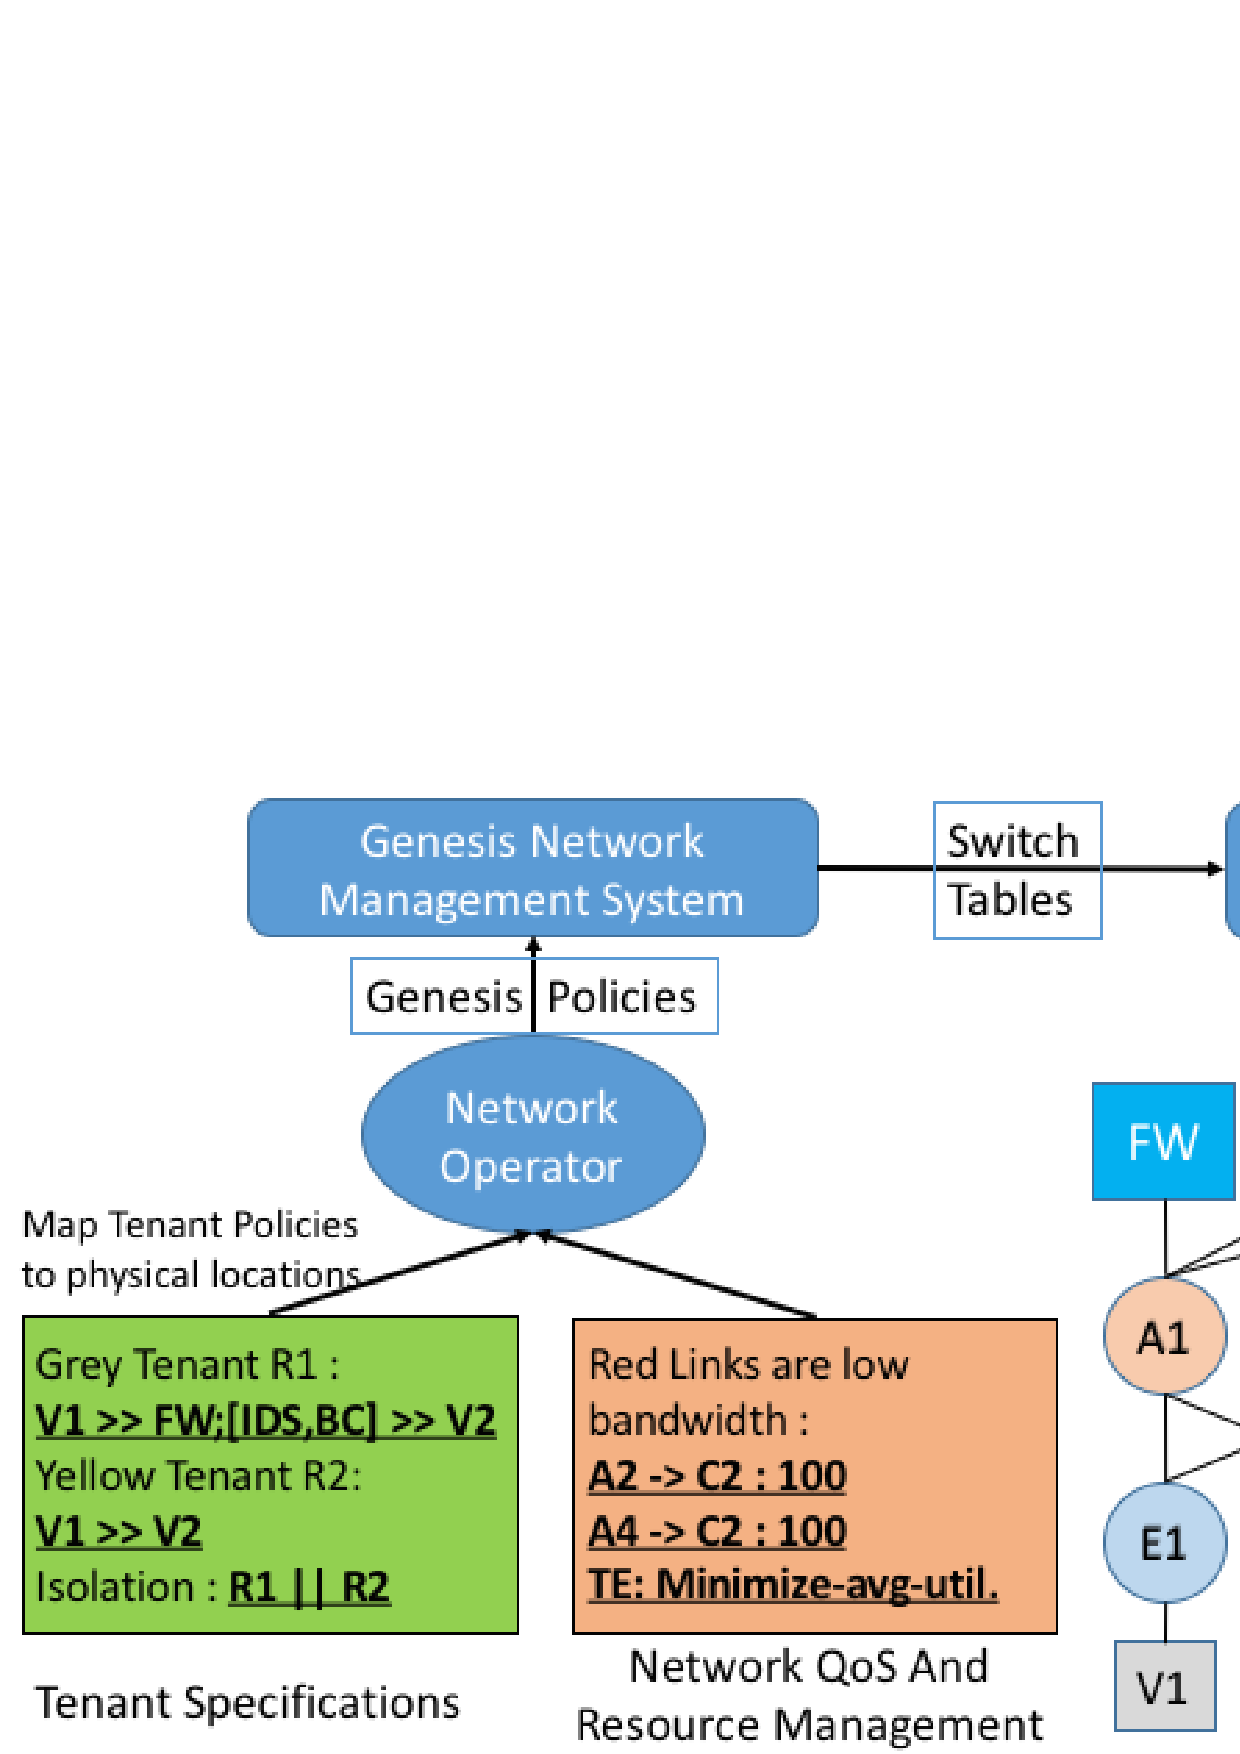
\includegraphics[width=\columnwidth]{figures/architecture.pdf}
\compactcaption{Two-phase process for generating a control plane
       with failure-tolerance properties}
\label{fig:architecture}
\end{figure}

\minisection{Configuration Synthesis}
To address the following challenges, we propose
\emph{automatic synthesis} of configurations, such that 
the network forwarding behaviour of the distributed
control plane meets policy specifications. 
Unfortunately, this task is inherently challenging 
as it requires solving in one shot multiple
computationally hard problems.
For example, even when considering 
static routing and no failures, 
synthesizing configurations 
that satisfy policies 
such as isolation and waypoints
is an NP-hard problem~\cite{genesis}.
Although the progress in SMT solving 
has made many NP-hard problems more practical, 
attempts of incorporating concepts such 
as shortest path algorithms 
into these solvers have resulted 
into huge performance losses~\cite{monosat}, 
not suited for real-world networks.

Our proposed approach is to tackle these problems 
in separate phases
(\figref{fig:architecture}).
First we synthesize a data plane that 
meets the input policies (\secref{sec:genesis}).
Using the data plane as input 
to the second phase, we 
express the problem of 
finding router configurations which 
induce the data plane provided by the
first phase using distributed routing
protocols (OSPF, BGP). Our contribution 
is \name, a framework for synthesizing
router configurations from the data
plane (paths) as input. 

\minisection{OSPF Synthesis}
For the OSPF protocol, configurations assign
weights to links between routers (directed edges
in the network topology). When the network has
to forward a packet from $s$ to $t$, the
OSPF routers uses 
Djikstra's algorithm to chose the
shortest weighted path from $s$ to $t$. Thus,
given input paths, \name finds edge weights 
(which are global for all paths) such that 
the shortest path through the network
for these endpoints exactly match the input paths. 
For example in \Cref{fig:ospfexample}(a), if the input
path is $s\rightarrow r_1 \rightarrow t$ for
destination IP $\lambda$, \name assigns
edge weights such that the input path has a strictly
smaller weight ($w=1+2$) than the other path $s \rightarrow t$ 
($w=5$). Thus, the OSPF routers will forward traffic for
$\lambda$ from $s$ to $t$ through $r_1$. \name 
efficiently computes weights by generating constraints
in the theory of Linear rational arithmetic (LRA) and
uses fast off-the-shelf LP Solvers 
(\secref{sec:ospfsynthesis}). 

However, given a set of paths as input, there may
not exist a solution to the edge weights. Consider the 
input paths as shown in \Cref{fig:ospfexample}(b). 
Both the red and blue paths are required 
to be the unique shortest path between $s$ to $t$
and, clearly, this is cannot be enforced for any 
choice of the edge weights (as weights correspond 
to all destinations). 
One way to synthesize configurations in this scenario 
is to ``disable'' the edge
$(s, t)$ for destination $\lambda_1$.
Using this technique, 
there is only one possible path from $s$ to $t$
for destination $\lambda_1$ ($s\rightarrow r_1 \rightarrow t$),
therefore is chosen as the shortest path. For 
destination $\lambda_2$, the $s\rightarrow t$ path
has a smaller weight ($w=1$) than the
$s\rightarrow r_1 \rightarrow t$ path ($w=1+2$), therefore,
both traffic is forwarded through the input paths for
both the destinations. 
This blocking mechanism is called a route-filter, and
we modify \name's OSPF synthesis algorithm to support
route-filtering (\secref{sec:filtering}).
 

\begin{figure}
	\centering
	\subfloat[Edge Weights]{
		\raisebox{0.5cm}{\resizebox {0.5\columnwidth} {!} {
	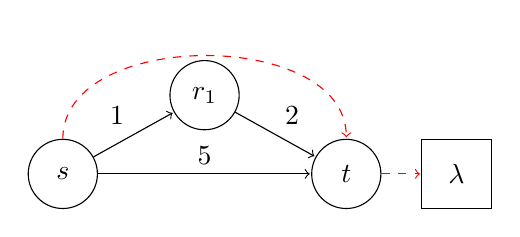
\begin{tikzpicture}[shorten >=0.5pt,node distance=,on grid,auto,
	square/.style={regular polygon,regular polygon sides=4}] 
	\node[state] at (0,0) (s)  {$s$}; 
	\node[state] at (1.8,1) (v1)  {$r_1$}; 
	\node[state] at (3.6, 0)(t) {$t$};
	\node[state, rectangle] at (5, 0) (d1) {$\lambda$};
	\path[->] 
	(s) edge node {1} (v1)
	edge  node {5} (t)
	edge [red, dashed, bend left=90] node {} (t)
	(v1) edge node {2} (t)
	(t) edge [red, dashed] node {} (d1);
	\end{tikzpicture}
	}}}
	\subfloat[Route-Filters]{
			\resizebox {0.5\columnwidth} {!} {
		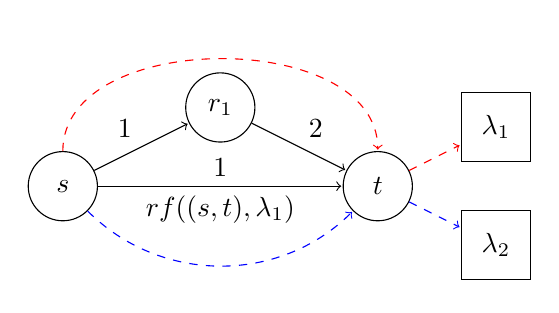
\begin{tikzpicture}[shorten >=0.5pt,node distance=,on grid,auto,
		square/.style={regular polygon,regular polygon sides=4}] 
		\node[state] at (0,0) (s)  {$s$}; 
		\node[state] at (2, 1) (v1)  {$r_1$}; 
		\node[state] at (4, 0)(t) {$t$};
		\node[state, rectangle] at (5.5, 0.75) (d1) {$\lambda_1$};
		\node[state, rectangle] at (5.5, -0.75) (d2) {$\lambda_2$};
		\path[->] 
		(s) edge node {1} (v1)
		edge  node [above] {1} node [below] {$rf((s,t),\lambda_1)$} (t)
		edge [red, dashed, bend left=90] node {} (t)
		edge [blue, dashed, bend right=45] node {} (t)
		(v1) edge node {2} (t)
		(t) edge [red, dashed] node {} (d1)
		(t) edge [blue, dashed] node {} (d2);
		\end{tikzpicture}
	}}
	\compactcaption{Example of paths which require route-filtering. This is a
		diamond starting at $s$ and ending at $t$. The diamond can be
		eliminated by filters $((s,r_1),\lambda_2)$ or $((s,r_2),\lambda_1)$.}
	\label{fig:ospfexample}
\end{figure}



\minisection{Dynamic Domain assignment}
The OSPF routing protocol does not scale 
with increasing network sizes
as it uses reliable
flooding of link-state packets. Flooding 
of updates can  
overwhelm the network when links fail. 
Ideally, operators would want to specify
limits on the size of an OSPF routing domain. 
Thus, a network could be 
split into multiple continuous OSPF domains,
which exchange routes across domains using
a inter-domain protocol like BGP.

We augment \name to synthesize 
inter-domain routing configurations 
such that each router is assigned to
a particular domain. 
Each domain is continous (all routers
are reachable to one another) and 
uses OSPF for intra-domain routing.
Domains exchange routes among  
themselves using BGP, a path-vector 
protocol which primarily selects routes by 
the number of domains in the route. 
However, \name can 
use BGP's powerful path selection metrics 
like local preferences such that  
paths with greater path lengths are selected.
OSPF has better convergence times than BGP,
thus, it is advantageous to use OSPF for 
routing in small domains and using BGP for
inter-domain routing. 

We consider the network to be managed by a 
single entity, therefore, the network can 
be split into domains\footnote{
The Internet is split into domains depending 
on ownership.} in numerous ways. Depending
on the network and input data plane, a certain
domain assignment of routers 
can optimize different metrics, like the
inter-domain configuration overhead (like BGP local
preferences and static routes) and OSPF route-filters
in the different domains. Thus, instead of operators
specifying a static domain assignment, \name stochastically
searches for the best domain assignment from the space of 
allowed assignments (for e.g., adhering to domain size limits)
to optimize different metrics. \name uses 
\emph{Markov chain Monte Carlo} sampling (MCMC) to perform
this stochastic search, and operators can specify parameters
to tune the cost function used in the search to assign priorities
to different metrics. 

\todo{Write about paper outline}





%ailures that happen in the later phases may require to restart the synthesis procedure 
%multiple times.
%but preliminary results of our approach are promising.


%The solution space of output network configurations to 
%enforce a set of policies
%is large; configurations can use different 
%network protocols (e.g., only BGP, only OSPF or a hybrid) and
%mechanisms (e.g., route filters, access control lists
%or protocol-specific variables). The large solution space
%of configurations complicates the synthesis of
%network configurations from
%input policies, 
%or ties the synthesis to a particular type of configuration. 
%Instead, we borrow a page from programming languages
%research and
%synthesize an Abstract Representation for Control planes (ARC)~\cite{arc} 
%from the data plane; the ARC can then be translated to actual device configurations.
%The ARC uses the notion that most routing protocols in use 
%today employ a cost-based path selection algorithm; thus a weighted
%graph can be used to abstractly represent the control plane such that 
%the path between two points taken in the network would be 
%the lowest weight path in the graph. 
%The ARC effectively decouples the policy component with the 
%actual network infrastructure. 

% While we use an abstract representation of the control
% plane (ARC) to simplify the synthesis, operators need control 
% planes conforming to certain requirements of the 
% underlying network infrastructure. For example, a 
% network may comprise of switches which do not have custom
% features like ACLs or route-filters, thus the ARC must take 
% into consideration these requirements. Without losing 
% generality, we translate these 
% requirements as types of ARCs with different properties,
% and still use a protocol-independent representation
% to represent the control plane. 

% In this paper, we primarily focus on 
% the second and third phase of our architecture, 
% i.e synthesizing a control plane from a set 
% of input paths and transforming the control plane to 
% satisfy policies under failure scenarios. The first 
% phase has seen promising work in recent times~\cite{merlin,
% simple}, these systems generate data planes to enforce 
% different kinds of policies, and 
% we can be retrofit these systems to generate different 
% data planes to integrate in our three-phase approach.

% thus, the networking infrastructure could be
% transitioned to different protocols without affecting the policy 
% control of the architecture. From the ARC, we can construct different
% drivers for translation to actual device configurations; these drivers
% can leverage inferences from healthy network practices in 
% real-life networks~\cite{mpa-imc15} to produce ideal network configurations.


%\aaron{Old text below}
%
%To tackle synthesis 
%of distributed control planes, 
%we use as input the network data plane 
%(set of forwarding paths) \aaron{Where does this data plane come from and
%    why is it reasonable to assume an operator can provide one?} which 
%enforces the operator-specified policies to
%synthesize an abstract representation of the control plane
%called ARC. \aaron{Our approach (ARC) should not come up until later in the
%    motivation, if at all.}
%The advantage of using network data planes as 
%input is the ease of developing
%different network management applications 
%enforcing proactive policies\footnote{
%Traditional control planes cannot support reactive policies, however
%middleboxes can overcome this limitation.} 
%as if operating over a software-defined
%network, agnostic of the actual network protocols used in the network.
%\aaron{I don't understand the preceding sentence. I'm still not clear why you
%take a single data plane as input and not multiple data planes or just the
%policies. I realize it is hard to synthesize from the latter, but can you be
%more precise why it is hard?}
%Many existing network management systems like Merlin~\cite{merlin} 
%and SIMPLE~\cite{simple}\footnote{
%Traditional control planes cannot support 
%paths with loops for service chaining.} developed for SDNs 
%could be seamlessly integrated to the architecture with minimal changes.
%\aaron{Do we need the preceding sentence?}
%Thus, using the data plane as input, we synthesize a control plane
%such that the paths decided by the control plane are the same 
%as the data plane input, and these paths satisfy the operator 
%policies.
%
%However, the control plane does not guarantee policy compliance 
%when failures occur. For
%example, if a link along the shortest path 
%%(\aaron{refer to some example figure}) 
%fails, \aaron{Need to mention earlier that we assume shortest-path-based route
%computations, ala OSPF} the next shortest path will become the new path to reach the
%destination. The control plane automatically computes the new shortest path
%(assuming one exists), thus preserving connectivity. 
%However, the new path may
%not conform to the same policies as the path in the 
%original failure-free data
%plane from which the control plane was synthesized: 
%e.g., the new path may no longer
%traverse a waypoint or have the same bandwidth capacity. Thus,
%synthesis must take into account policy-compliance under failures.
%
%Policy-compliance under failures is difficult to achieve due 
%to the large number of failure scenarios to consider and can 
%be impossible to synthesize a control plane which is 
%policy-compliant under all failures. Operators require 
%varying degrees of policy-compliance under failures for 
%which we propose two classes of policies: {\em hard} and
%{\em soft} policies. Operators can specify 
%hard policies pertaining
%to security are of the utmost importance, 
%because they protect the network and
%its services from attacks and unauthorized accesses. Some 
%examples of hard policies are as follows: 
%a particular flow must always traverse through a waypoint 
%under any failure scenario, or a certain pair of hosts must 
%never be able to communicate (always blocked). 
%Soft policies can be considered as objectives which improve 
%the control plane, but are not strict requirements, typically
%pertaining to performance. The consequences of violating
%soft policies are less severe. Operators can provide 
%backup paths for flows (generated such that they 
%satisfy the data plane policies) as soft policies, 
%and the synthesis of the control plane 
%tries to satisfy as many soft policies as 
%possible. 
%
%\aaron{Discussion of the available control plane constructs should come up
%    earlier.}
%While we use an abstract representation of the control
%plane (ARC) to simplify the synthesis, operators need control 
%planes conforming to certain requirements of the 
%underlying network infrastructure. For example, a 
%network may comprise of switches which do not have custom
%features like ACLs or route-filters, thus the ARC must take 
%into consideration these requirements. Without losing 
%generality, we translate these 
%requirements as policies determining the properties of the
%ARC, and thus, still use a protocol-independent representation
%to represent the control plane. 
%
%Our architecture envisions network operator providing
%a policy-compliant data plane and a set of hard and soft policies
%pertaining to policy-compliance under failure and network 
%infrastructure requirements as input to synthesize resilient 
%control planes. Towards this vision, we present  
%approaches to synthesize different types of the ARC and the 
%challenges involved in making synthesis efficient and
%extending these approaches to support a wider range of 
%policies and functionalities. 

\section{Example}
Consider the hierarchical network in \cref{fig:example} which
is split into three OSPF domains, and these domains communicate
using BGP. Host A talks to host B and C with the following policies:
traffic to B must go through a firewall at router $r_4$ and traffic 
to B and C do not share any links (We discuss the policy support in
detail in \Cref{sec:policy}). Given the particular domain assignment, 
we have to synthesize OSPF and BGP configurations satisfying the 
following policies. Illustrating our two-phase approach, we first 
use Genesis to find policy-compliant paths (indicated by the blue and
red paths). Note that there exists multiple solutions for the given
policies, we show how the control plane is 
synthesized using one of the solutions:

\begin{itemize}
	\item
For traffic $A \rightarrow B$, the entire path is inside
a single OSPF domain, so Zeppelin has to find OSPF weights 
such that the shortest path is $r_1 \rightarrow r_3 \rightarrow 
r_2$. \Cref{fig:example} shows the OSPF weights which induce
this path, we can see that the weight of path $r_1 
\rightarrow r_3 \rightarrow r_2$ () is greater than that of path
$r_1 \rightarrow r_2$ (). 
 	\item For traffic $A \rightarrow C$, the path traverses through 
 	multiple domains, so Zeppelin configures BGP so as to ensure
 	routing through domains follows the Genesis path. In this case, 
 	we need traffic to go through a longer path in terms of AS path
 	length; Zeppelin sets $r_4$'s BGP local preference for route C
 	from $r_5$ a higher value (200), so that $r_5$ is 
 	preferred over $r_6$. 
 	\item Suppose the operator wanted to compute better domain
 	assignments for the network. We can see that if $r_5$ was moved
 	to $D_2$, we do not even need to configure the local preference 
 	at $r_4$, thus, simplifying the BGP configuration complexity. 
 	Zeppelin can find better domain assignments using a stochastic
 	search procedure. 
\end{itemize}
\section{Routing Model and Problem Definition}
In this section, we formally define the problem addressed in this
paper.  We first define how different
routing protocols are represented.  In particular, we model static
routes, OSPF shortest-path routing, and BGP preference-based routing.
Then, we formally define when a certain configuration meets a given
set of policies and present the configuration synthesis problems
we tackle.

\subsection{Routing Model}

\minisection{Preliminaries}
We represent the physical router topology as a directed graph $T=(V, L)$,
where $V$ is the set of routers and $L\subseteq V\times V$ is the set of links. 
Throughout the paper we assume $T$ is fixed.
We use the neighbour function $N(s) = \{s'\ | \ (s,s') \in L \}$ to denote 
the set of neighbour routers of $s$. 
We define $\Lambda$ to denote the set of destination IP subnets;
distributed protocols make forwarding decisions based on the 
destination address/subnet (see Figure~\ref{fig:ospfexample}).

A path $\pi = (u_1,v_1) (u_2, v_2) \cdots (u_n, v_n) \in L^*$ is a loop-free valid path if
a  vertex is not visited more than once---i.e.,
$u_1\neq v_n\wedge\forall i,j \leq n. 
~i \not= j \rightarrow u_i \not= u_j$---and adjacent links in the
path share a router---i.e., $\forall i < n. ~v_i = u_{i+1}$.
Sometimes we represent the path $\pi$ as $u_1\rightarrow u_2 \rightarrow  \cdots \rightarrow v_n$.
Given two nodes $s$ and $t$, we use $\Pi_s^t$ to denote the set of all paths
with source $s$ and target $t$---i.e., $u_1=s$ and  $v_n=t$. 
We write $l \in \pi$ when the path $\pi$ contains the link $l$. 

To model hierarchical control planes in which
 the network is divided into continuous domains,
we define a router domain assignment function
$\Theta: V \rightarrow \nat$ which maps each router to a domain 
(denoted by a natural number).
Each domain uses OSPF as the intra-domain routing protocol
and BGP as the inter-domain routing protocol. 


The OSPF configurations are expressed 
using two functions: edge weights $W$ and
 route filters $RF$. For BGP configurations: 
we have the local preference function $LP$ 
and the iBGP filter function $IF$. Static 
routes are expressed using the $SR$ function.
We express the complete network configuration $C$
as a tuple $(\Theta,W,RF,LP,IF,SR)$.  In the 
rest of the section, we describe each component 
of the configuration $C$ and the routing function 
$\route^C$ for the network given the configuration $C$. 
We assume the following  
simplifying property for $C$: for any two 
routers $r_1$ and $r_2$,
traffic will be forwarded from $r_1$ to $r_2$ 
along a single path. 
When synthesizing $C$, we will ensure that this property is satisfied.


\minisection{Static Routes} Static routing refers to a router using a
manually-configured routing entry, rather than information from
dynamic protocols like OSPF or BGP.  Static routing is useful to enforce certain
paths that are not easily realizable using routing protocols because 
static
routes for a given destination have the highest preference over other routes for the same
destination.  
We define the static route partial
function $SR: V \times \Lambda \mapsto V$ with the following meaning. 
Given a router $r$
and destination $\lambda$, if $SR(r,\lambda)=r'$, then traffic for
destination $\lambda$ reaching node $r$ is always forwarded to node
$r'$. We assume that  the static routes induced by the function $SR$ form paths and
we use $\Pi_{SR}$ to denote the set of all  static paths. 
Formally, for a destination $\lambda$ and a router $r$, if $SR(r,\lambda)=r'$ then
either $r'$ is directly connected to the subnet $\lambda$ or there exists $r''$ such that $SR(r',\lambda)=r''$.

%These paths would have a highest preference.

\minisection{OSPF} Open Shortest Path First (OSPF) is a routing
protocol commonly used inside a domain. Each router receives link
state information from other routers and uses this to create a map of
the network. Positive weights are defined for each link in the
network, and each router used Djikstra's algorithm to forward to the
destination along the weighted shortest path to the router the
destination   is connected to.

Let us
define the OSPF weight function $W: L \rightarrow \rat$ which 
maps edges of the topology to positive rational weights. 
% todo: When to talk about converting LRA to LIA.
For a given
path $\pi=l_1\ldots l_n$, we indicate the sum of weights of the
links in the path by $W(\pi)=\sum W(l_i)$. 


We allow  route filters
to selectively disable an
edge for a given destination by  
blocking advertisements to a
particular destination along a link. 
Formally, a  route filter is a pair $(l,\lambda)\in L\times \Lambda$
which disables the link $l$ for destination $\lambda$. 
We define the  route filter function 
$RF: \Lambda \rightarrow 2^L$ which maps each destination  
to a set of filtered links in the topology. 
Given an   destination $\lambda\in \Lambda$, 
a legal path with respect to $RF$ and $\lambda$
is a valid path $\pi=l_1\cdots l_k$ such that for every $i$,
$l_i\not\in RF(\lambda)$.
We use $\Pi_\lambda$ to denote the set of all such paths.

We define the routing function 
$\route_{ospf}^G$ 
that given 
%a weight function $W$,
%a  route filter function $RF$,
a source node $s$,
a target node $t$,
and destination   
$\lambda$,
returns the OSPF-induced paths from $s$ to $t$ for destination   $\lambda$.
The paths between two nodes are
the shortest paths in the network
that do not cross any link that belongs to $RF(\lambda)$. We also
account for the higher priority of static routes.
\[
\route_{ospf}^C(s,t,\lambda) = 
\begin{cases}
\pi  & \text{$\Pi_s^t \cap \Pi_{SR} =\{\pi\}$} \\
\pi & 
\text{$\Pi_s^t \cap \Pi_{SR} =\emptyset \wedge \pi\in \Pi_s^t\cap \Pi_\lambda ~\wedge $}  \\
& \text{~~~~$\neg\exists \pi'\in\Pi_s^t\cap \Pi_\lambda . W(\pi')< W(\pi)$} 
\end{cases}
\]

\minisection{BGP} BGP is a path-vector inter-domain routing protocol
that connects different autonomous systems (ASes), where each AS
comprises of one or more routers (typically managed by a single
entity). A BGP router receives routes from BGP peers (internal peers
send iBGP routes, external peers send eBGP routes). Each route for the
destination comprises of a domain-level path to the destination
domain, and by default a BGP router will pick a path with fewest domains 
to forward the packet for a destination.
 
To support policy routing, BGP routers can be configured with a
\emph{local preference} variable to assign higher priorities to
specific routes for a particular destination. We define the local
preference function $LP: V \times V \times \Lambda \mapsto \nat$ as
follows.  Given a BGP router $r$, neighbouring router $r_1$, and  
destination $\lambda$, $LP(r, r_1, \lambda)$ specifies the local
preference for a route received for destination $\lambda$ at BGP
router $r$ from next-hop BGP router $r_1$.  This function is defined
on inter-domain links.  From the routes received at $r$, the router
picks the route with greatest local preference.

The Internal BGP (iBGP) protocol is used to 
exchange external BGP routes 
among BGP routers belonging
to the same domain. A external route received 
by $r_1$ with a local preference value configured 
will be advertised to the rest of the BGP routers of the 
domain as an iBGP route with the same local
preference. We can configure iBGP 
filters to prevent a router from advertising 
a route to another router. We do so using the 
function $IF: V \times \Lambda \mapsto 2^V$;
if a BGP router $r_1 \in IF(r_2, \lambda)$, then
$r_2$ will not advertise a route for $\lambda$ to
$r_1$ through iBGP. 
 
 \iffull
Algorithm~\ref{alg:bgppathrules} defines the routing function 
$\route_{bgp}^C$ 
that given 
%a local preference function $LP$,
a BGP router $r$
and destination  
$\lambda$,
returns 
the next-hop BGP router in the path. 
\else
We only describe the routing semantics of BGP
informally. The BGP path selection algorithm is submitted as part of the supplementary material.
\fi
BGP 
chooses a route with highest local preference, and
if there is a tie, it then chooses the route with smallest
AS path length~\cite{bgp}. 
\name synthesizes configurations where all ties are 
are broken using these criteria, and $\route_{bgp}^C(r,\lambda)$
returns a single router for the inter-domain next-hop router. 
Also, static routes 
have a higher preference than BGP, therefore a static route
$SR(r, \lambda)$ will be preferred over the BGP route.

\iffull
\begin{algorithm} [t]
	\begin{footnotesize} 
		\caption{BGP Best Path Selection at router $r$ for dst. $\lambda$}
		\label{alg:bgppathrules}
		\begin{algorithmic}[1]
			\Procedure{BestPath}{} \\
			\hspace*{0.4cm} [Each route $\gamma$ of form $(\lambda, local\_pref, len, nexthop)$]
			\State{$\Upsilon_{ebgp}$ = $\bigcup$ Route from external BGP neighbour for $\lambda$} 
			\State{$\Upsilon_{ibgp}$ = $\bigcup$ Route from internal BGP router $r_1$:
				 $r \not\in IF(r_1, \lambda)$}
			\State{$\Upsilon = \Upsilon_{ebgp}\cup \Upsilon_{ibgp}$}
			\\
			\If{$SR(r,\lambda) = r_1$} 
			\State{$\route^C_{bgp}(r, \lambda) = r_1$\hfill [Static Route has highest pref.]}
			\Else \\
			\indent\indent \hspace{0.3cm}[Find routes with highest \emph{local preference}]
			\State{$\Upsilon_{lp} = \{\gamma \in \Upsilon \mid \forall \gamma_1 \in \Upsilon. ~\gamma.local\_pref \geq \gamma_1.local\_pref\}$}
			\If{$|\Upsilon_{lp}| = 1$}
			\State{$\gamma_{best} = \gamma \in \Upsilon_{lp}$}
			\Else \newline
			\hspace*{0.7cm}\indent [Prefer the path with the smallest \emph{AS Path length}]
			\State{$\Upsilon_{as} = \{\gamma \in \Upsilon_{lp}  \mid \forall \gamma_1 \in \Upsilon_{lp}. ~\gamma.len \leq \gamma_1.len\} $}
			\If{$|\Upsilon_{as}| = 1$}
			\State{$\gamma_{best} = \gamma \in \Upsilon_{as}$}	
			\EndIf
			\EndIf
			\If{$\gamma_{best} \in \Upsilon_{ebgp}$}
			\State{$\route^C_{bgp}(r, \lambda) = \gamma_{best}.nexthop$}
			\State{Redistribute $\gamma_{best}$ to OSPF domain}
			\Else \\
			\hspace*{0.7cm}\indent [Traffic for $\lambda$ will not exit domain through $r$]
			\State{$\route^C_{bgp}(r, \lambda) = \bot$}
			\EndIf
			\EndIf
			\EndProcedure
			%				\State{ . }
			%				\State{Prefer the path with the lowest \emph{multi-exit discriminator} (MED).}
			%				\State{Prefer eBGP over iBGP paths.}
			%				\State{Prefer the route that comes from the BGP router with the lowest \emph{router ID}.}
		\end{algorithmic}
	\end{footnotesize}
\end{algorithm}
\fi

\minisection{OSPF+BGP+Static Routes} We now describe how routing
happens across domains.  In domain $d$, traffic 
for destination $\lambda$ originates at source
router $s$ (i.e., $\Theta(s) = d$). 
If the target router $t$ connected to the
destination belongs to domain $d$, then there exists a OSPF route for
$\lambda$ at $s$, and the path taken would be
$\route_{ospf}^C(s,t,\lambda)$.

Consider the case of destination $\lambda$ being connected 
to an external domain, thus, traffic for destination $\lambda$
will be sent to a BGP gateway router of domain $d$ which 
will forward it to its neighbouring domains till
it reaches the internal domain of $\lambda$. A BGP gateway
router is a router $g$ such that $\exists g' \in N(g). 
~\Theta(g') \not= \Theta(g)$. 

However, not all BGP routes for $\lambda$
are distributed 
into OSPF (to prevent explosion of forwarding tables). 
BGP gateways in a domain exchange routes using iBGP,
and if the best path chosen is an eBGP route, 
the gateway redistributes the eBGP route into OSPF. 
Therefore, multiple BGP routers
can redistribute a route for $\lambda$,  
the closest gateway (in terms of OSPF distance)
is chosen. We define a gateway function $G^C$,
that given a domain number $n\in \nat$
%a local preference $LP$,
%a weight function $W$,
%route filters $RF$,
a router $r$ such that $\Theta(r)=n$,
and destination $\lambda$ outside of domain $n$, 
specifies the
gateway chosen for a destination based on the
closest router redistributing the route for $\lambda$. 
Finally, the routing function 
$\route^C$
%:\Theta \times LP \times W \times RF \times V \times V \times \Lambda \rightarrow L^* 
returns paths from source to destination in a inter-domain network:
given a source $s_1$ and a destination $\lambda$ connected to target router $t$, 
\[
\begin{array}{c}
	\route^C(s_1, t, \lambda) = 
	\route_{ospf}^C(s_1,g_1, \lambda) + 
	 (g_1, s_2 )+\qquad\qquad\qquad  \\
%	~~~~~~~~~~~~~~~~~~~~~~~~~\route_{ospf}^C(s_2,g_2, \lambda) + (g_2, s_3) + \\
	\qquad\qquad\qquad\qquad \ldots  + (g_{n-1}, s_n) +\route_{ospf}^C(s_n,t,\lambda)
\end{array}
\]
Here, for each $i>1$, $g_i=G^C(\Theta(s_i),s_i,\lambda)$, 
$s_i=\route_{bgp}^C(g_{i-1}, \lambda)$,
and  $+$ is the concatenation operator for paths. 

\minisection{Induced paths}
We assume a set of packet classes $PC : [0,C_{pc}]$ 
and map each path (only reachability policies produce paths,
the rest specify properties on these paths)
to a unique integer in $PC$.
For a packet class $pc$, $src_{pc}$ denotes the source router,
$dst_{pc}$ denotes the destination router, and $\lambda_{pc}$
denotes the destination   address. 


\begin{definition}[Induced Paths]
Given a configuration $C$ and a set of packet classes $PC$, the set of paths
$\paths^C(PC)$ induced by $C$ is defined as follows: 
$\forall pc \in PC.$ $\route^C(src_{pc}, dst_{pc}, \lambda_{pc})$ $\in \paths^C(PC)$.
\end{definition}

\subsection{Problem Definition}
\begin{table}
\begin{small}
	\begin{center}
		\begin{tabular}{m{7.8em}  m{15.9em} } 
			{\bf Policy} & {\bf Description} \\ 
			\hline
			Reachability & There is a path from router $s$ to router $t$ for destination $\lambda$ \\ \hline
			Reachability with \newline Waypoints & The path  from $s$ to $t$ for destination $\lambda$ 
			traverses a set of waypoints in the path\\ \hline
			Traffic Isolation & Paths of two reachability policies $R1$ and $R2$ do not share  links \\ \hline
			Traffic Engineering  & Minimize total/max link utilization \\
		\end{tabular}
	\end{center}
	\caption{\genesis path-based policy support.} \label{tab:policysupport} 
\end{small}
\end{table}
\begin{table}[!t]
	\begin{small}
		\begin{center}
			\begin{tabular}{m{6.5em}  m{17.7em} } 
				{\bf Policy} & {\bf Description} \\ 
				\hline
				Count  & Number of OSPF domains: $c_1\leq N_D\leq c_2$  \\ \hline
				Domain Size  & Lower and upper
				limit of size of domain (number of routers): $l\leq ds\leq u$ \\ \hline
				BGP \newline Enable & Enable BGP on routers $B$ (hardware constraint) \\ \hline
				Static Route: ${sc}$ & Upper bound number of static route rules: $sc < C_{sc}$ \\ \hline
				BGP Config. Overhead: $bc$ & Upper bound the number of local preference entries and iBGP filters $bc < C_{bc}$ \\ \hline
				Cost Minimization & Minimize user-defined cost $expr(sc, bc)$
			\end{tabular}
		\end{center}
		\caption{\name configuration policy support.} \label{tab:configpolicysupport} 
	\end{small}
\end{table}
\begin{table}[!t]
\begin{small}
	\begin{center}
		\begin{tabular}{m{6.5em}  m{17.7em} } 
			{\bf Policy} & {\bf Description} \\ 
			\hline
			Count  & Number of OSPF domains: $c_1\leq N_D\leq c_2$  \\ \hline
			Domain Size  & Lower and upper
			limit of size of domain (number of routers): $l\leq ds\leq u$ \\ \hline
			BGP \newline Enable & Enable BGP on routers $B$ (hardware constraint) \\ \hline
			Route-Filters: $rc$ & Lower bound number of filters:
			$rc > C_{rc}$\\ \hline
			Static Route: ${sc}$ & Upper bound number of static route rules: $sc < C_{sc}$ \\ \hline
			BGP Config. Overhead: $bc$ & Upper bound the number of local preference entries and iBGP filters $bc < C_{bc}$ \\ \hline
			Cost Minimization & Minimize user-defined cost $expr(rc, sc, bc)$
		\end{tabular}
	\end{center}
	\compactcaption{\name configuration policy support.} \label{tab:configpolicysupport} 
\end{small}
\end{table}


\minisection{Policies}
\Cref{tab:policysupport} describes the path policies supported by \name.
Given  a set $\Psi$ of
path policies, we say that
a set of paths $\Pi$ is policy-compliant with respect to $\Psi$, $\Pi \models \Psi$,
if the paths in $\Pi$ satisfy all the policies in $\Psi$ (see~\cite{genesis} for the formal definition). 


\Cref{tab:configpolicysupport} describes all the configuration policies supported by \name.
A configuration $C$ satisfies a set of configuration policies $P$
if $C$ satisfies every constraint in $P$.
For each configuration policy 
we define what it means for  a configuration $C=(\Theta,W,RF,LP,IF,SR)$ to satisfy it.

The first type of policy restricts how many OSPF domains $N_D$ a
configuration might have, $c_1\leq N_D\leq c_2$ 
and it is satisfied by $C$ iff $c_1\leq |\{\Theta(r)\mid r\in V\}|\leq
c_2$.  This policy is useful for avoiding situations resulting in too
many domains in the hierarchical split which can be difficult to
administer.  The second type of policy allows the operator to restrict
the size $k$ of each OSPF domain, $l\leq k\leq u$, because OSPF does
not scale gracefully with network size.  This policy is satisfied if
for every domain $i$, $l\leq |\{r \mid \Theta(r)=i\}|\leq u$.


Certain 
	routers may not be suited to run BGP due to resource
	constraints. Thus, the operator can specify what set of 
	routers $B\subseteq V$ is BGP compatible.  
	This policy is satisfied if none of the routers $V\setminus B$
	is a gateway router.
	Formally, for every $r\in V\setminus B$,
	there doesn't exist a router $r'\in N(r)$ such that $\Theta(r) \not= \Theta(r_1)$

Finally, \name provides ways to specify upper bounds on the number of
1) route filters, which in general reduce the resiliency of the network---i.e., $rc=|\cup_{\lambda\in \Lambda} RF(\lambda)|\leq C_{rc}$,
2) static routes---i.e., $sc=|\{(v,\lambda)\mid \exists v'. SR(v,\lambda)=v'\}|\leq C_{sc}$, and
3) BGP configurations, which increase the complexity of the network---i.e., 
$bc=|\cup_{v,\lambda\in V\times\Lambda} IF(v,\lambda)\cup \{(v,v',\lambda)\mid LP(v,v',\lambda)\neq \bot|\leq C_{bc}$.
\name also allows to minimize certain expressions over the quantities $rc$, $sc$, and $bc$---e.g., $max(rc, sc+bc)$. 
Ideally, the most important metric we want to maximize is resiliency---i.e.,
the number of alternate paths between endpoints.
However, this metric is too hard to handle as it depends on complex graph properties. 
In practice, when we want improve resiliency, we try to minimize
the number of filters; we will show that this strategy is effective. 

%different configuration metrics. For example,
%we allow  route filters in OSPF synthesis 
%(\secref{sec:ospfsynthesis}), which may yield undesirable
%endpoint resilience, thereby, synthesizing configurations
%which provide a specified metric of resilience or maximize
%the metric. Similarily, to enable path-based inter-domain routing, 
%\name needs	to set up static routes along the path, or configure BGP 
%variables like local preferences to ensure the configurations 
%induce the input paths.
%These increase the size of the configurations,
%thus increasing the complexity of verifying correctness either 
%manually or using verification tools~\cite{batfish, arc, era}. 
%Therefore,
%another objective \name considers is the configuration overhead
%to ensure path-compliance.



\minisection{Synthesis problems}
\noindent We can now define what it means for a configuration $C$ to be policy-compliant
and our synthesis problems.
\begin{definition}[Policy-Compliance] \label{def:policycompliance}
	Given a set of path policies $\Psi$ and a set of configuration policies $P$,
	the configuration $C$ is policy-compliant with $(\Psi,P)$,
	$C \models (\Psi,P)$, if the set of
	induced paths $\paths^C(PC) \models \Psi$
	and $C$ satisfies the policies in $P$.
	The \emph{configuration synthesis problem} is to find, given $\Psi$ and $P$,
a configuration $C$ that is policy compliant with $(\Psi,P)$.
\end{definition}

As anticipated in Section~\ref{sec:motivation}, our approach will proceed in two phases,
one of which solves the following sub-problem.  
\begin{definition}[Path-Compliance] \label{def:pathcompliance}
Given a set of configuration policies $P$,
and a set of paths $\Pi$ over packet classes $PC$,
	a configurations $C$ is path-compliant with 
	$(\Pi,P)$,
	if $\paths^C(PC)=\Pi$ and $C$ satisfies the policies in $P$.
	The \emph{path-compliance synthesis problem} is to find, given $P$ and $\Pi$,
a configuration $C$ that is path-compliant with $(\Pi,P)$.
\end{definition}




%We defined policy-compliance in terms of the 
%paths of the packet classes satisfying path-based 
%policies like isolation or traffic engineering. However,
%depending on the assignment of routers to different domains,
%the configurations generated may not be efficient
%in deployment. Therefore, we extend the notion of 
%compliance to policies on configurations 
%(\Cref{tab:configpolicysupport}).



%\section{Architecture} \label{sec:architecture}
In this section, we describe the architecture of our system.
Since directly generating policy-compliant configurations
is a challenging problem, we use a two-phase approach in which
we first synthesize policy-compliant \emph{paths}
using the tool \genesis~\cite{genesis} and then present
a new tool, \name, that synthesises configuration that produce the
paths we synthesized in the first phase. 
Since the first phase may produce \emph{bad} paths for which the
configuration synthesis is complicated or not possible,
we then propose ways to restart the algorithm by computing new paths.

\subsection{\genesis: From Policies to Paths} \label{sec:genesis}
The first phase of our approach produces a set of paths adhering to
different policies using \genesis~\cite{genesis}, a network management
system which synthesizes forwarding tables enforcing the policies. 
Some of the policies supported by \genesis are specified in 
\Cref{tab:policysupport}. 
Due to the rich policy language, generating policy-compliant paths is an NP-complete problem;
\genesis leverages fast off-the-shelf SMT solvers to provide
support for policy enforcement for a diverse set of policies.
Given a set of policies, \genesis generates a set of constraints 
over propositional logic (SAT) and Linear rational arithmetic (LRA),
such that the solutions to these constraints are forwarding
tables, which can be used to extract the 
policy-compliant paths.

\loris{two sentences about what \genesis currently does, 
generates constraints over Reach and Fwd and briefly mention meaning
of a solution}

\paragraph{Modifications from~\cite{genesis}}
In this section, we discuss how \genesis
constraints need to be modified to avoid generating paths that 
cannot be enforced by any routing configuration.

OpenFlow switches~\cite{openflow} support match predicates for
forwarding rules on different packet header fields like source
and/or destination IP address, ports etc. However, legacy protocols
like OSPF and BGP only support destination-based forwarding, 
forcing the paths to a destination subnet to 
form a directed tree rooted at the destination. 
Thus,
at any router, there exists at most one forwarding rule per destination. 
Since \genesis was built for
SDN management,  a switch may forward to different switches
packets that are directed to the same destination,
and thus cannot be induced by any router
configuration. 

We add constraints to \genesis to ensure that
if any two paths to a destination subnet intersect at a router,
the subsequent downstream paths to the destination from the
router do not \emph{diverge} at a router.  
\loris{assuming you have defined Reach and Fwd at 
earlier where I put comment}
We define the relation $Reach^*(sw,pc)$ to model reachability 
of $sw$ in the path of $pc$, i.e., it can be reached in zero or more
steps from the source. We can be expressed $Reach^*(sw,pc)$ 
in the network forwarding model of \genesis as:
\begin{equation}
	Reach^*(sw,pc) = \bigvee_{k \in [0, \mu]} Reach(sw, pc, k)
\end{equation}
$\mu$ denotes the synthetic limit of the length of the path. 
$Reach(sw, pc, k)$ is valid if $sw$ is reachable in the path of
class $pc$ in $k$ steps. Thus, to enforce the destination-based
forwarding using $Reach^*(sw,pc)$, we add
constraints for every pair ($pc_1$,$pc_2$) having the same 
 destination subnet:
 \begin{multline}
 \forall sw. Reach^*(sw, pc_1) \wedge Reach^*(sw, pc_2) \implies \\ \bigvee_{n \in N(sw)} Fwd(sw, n, pc_1) \wedge Fwd(sw, n, pc_2)
 \end{multline}
 $Fwd(sw_1, sw_2,pc)$ is valid if $sw_1$ forwards $pc$ to next-hop $sw_2$ and
 $N(sw)$ denotes the neighbours of $sw$. Basically, 
 if a switch is reachable for both packet classes, 
 then the next switch must be the same for both classes
 (paths will not diverge), and thus, the paths obtained
 from \genesis for a destination subnet will form a 
 directed destination tree. 

\subsection{\name: From Paths to Router Configurations} 
After we have computed a set of policy-compliant paths,
we need to solve the path-compliance problem using such paths.
To solve this problem, we propose the tool \name, which
combines techniques in constraint solving and randomized search
to efficiently generate router configurations for the paths obtained from \genesis.
For a given domain division of the network,
\name uses linear constraints to generate OSPF weights and BGP preferences.
If the constraints fail, \name uses the unsatisfiable cores to
identify where to place route-filters.
To decide how to split the network into domains,
\name uses Markov Chain Monte Carlo (MCMC) search to find
domain assignments that satisfy the configuration policies and have good resilience.
When the MCMC search does not progress and cannot find good solutions,
we restart the search by asking \genesis to generate a new set of paths.
These techniques are described in detail in the next two sections.

\section{Synthesising OSPF Configurations} \label{sec:synthesis}
In this section, we present an algorithm for 
solving the path-compliance problem for 
single-domain OSPF networks
---i.e., $|\{\Theta(n) \mid n\in V\}|=1$.

%\subsection{Complexity} \label{sec:rfcomplexity}

Before we present our technique and its intricacies,
we justify the complexity of our approach by showing that
the problem of synthesizing an OSPF configuration
that contains an optimal number of route-filters is NP-complete.

\begin{theorem}
Given a set of paths $\Pi$,
a topology $G=(V,E)$,
a domain-assignment function $\Theta$, such that $|\{\Theta(n) \mid n\in V\}|=1$,
a number $n\geq 0$,
the problem of finding 
an $LP$, $W$, and $RF$,  such that
\loris{PC shouldn't appear here, make consistent.}
$\paths(\Theta, LP, W, RF, PC) = \Pi$,
and 
$\sum_{\lambda\in\Lambda} |RF(\lambda)|=n$, is NP-complete.
\end{theorem}
\iffull
\begin{proof}
We show that the decision version of the minimum 
vertex cover problem, i.e., there exists a vertex cover
of size $ \leq k$, which is NP-complete, 
reduces to finding a set of route filters of size $ \leq k$ \
and OSPF weights for a network with only one domain. 
The latter is also in NP, so after the reduction we 
can conclude that it is also NP-complete.

Let $G = (V,E)$ be an instance of the 
minimum vertex cover problem. A set of
vertices $VC \subseteq V$ is the vertex cover
if $\forall (v_1, v_2) \in E. ~v_1 \in VC \vee v_2 \in VC$. 

We now show how to construct a topology $T=(S,L)$ 
and a corresponding set of paths $P$ that can be 
induced by route filter set $R$ such that $|R| \leq k$  
iff the corresponding $VC(R)$ is a vertex cover of 
the graph $G$ and $|VC(R)| \leq k$.

For every vertex $v \in V$: add two vertices $r_v^1$ 
and $r_v^2$ to $S$ and a directed link $r_v^1 \rightarrow r_v^2$ to $L$. 
We also assign a destination host $d_v$ for each vertex $v$. 

For every edge $(u,v) \in E$: add two vertices $s_{uv}$
and $t_{uv}$ to $S$. Add edges
connecting $s_{uv} \rightarrow s_{u}^1$, $s_{uv} \rightarrow s_{v}^1$,
$s_{u}^2 \rightarrow t_{uv}$ and $s_{v}^2 \rightarrow t_{uv}$. \Cref{fig:rfcomplexity} illustrates this construction.
\begin{figure}[H]
	\centering
	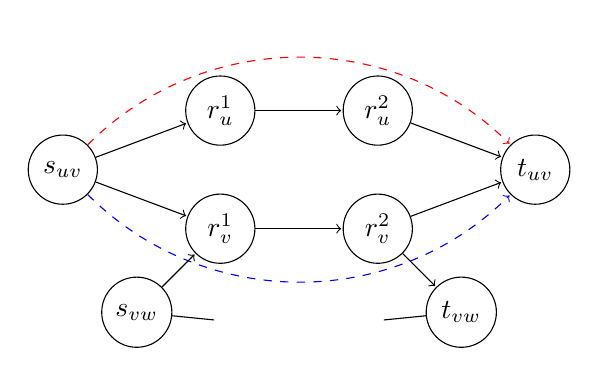
\begin{tikzpicture}[shorten >=0.5pt,node distance=1.5cm,on grid,auto,
	square/.style={regular polygon,regular polygon sides=4}] 
	\node[state] at (0,0) (s)  {$s_{uv}$}; 
	\node[state] at (2,-0.75) (v1)  {$r_v^1$}; 
	\node[state] at (4,-0.75) (v2)  {$r_v^2$};
	\node[state] at (2,0.75) (u1)  {$r_u^1$}; 
	\node[state] at (4,0.75) (u2)  {$r_u^2$}; 
	\node[state] at (6,0) (t) {$t_{uv}$};
	\node[state] (s1) [below left=of v1] {$s_{vw}$}; 	
	\node[state] (t1) [below right=of v2] {$t_{vw}$}; 	
	\path[->] 
	(s) edge  node {} (v1)
	edge  node {} (u1)
	edge [blue, dashed, bend right=45] node {} (t)
	edge [red, dashed, bend left=45] node {} (t)
	(u1) edge node {} (u2)
	(u2) edge node {} (t)
	(v1) edge node {} (v2)
	(v2) edge node {} (t)
	edge node {} (t1)
	(s1) edge node {} (v1);
	\path[-] (s1) edge node[above] {} +(1,-0.1);
	\path[-] (t1) edge node[above] {} +(-1,-0.1);
	\end{tikzpicture}
	\caption{Construction}
	\label{fig:rfcomplexity}
\end{figure}
If there was another edge $(v,w) \in E$, then
$s_{vw}$ has an edge connecting to $r_v^1$ and
$r_v^2$ has an edge connecting to $t_{vw}$ (shown
in \Cref{fig:rfcomplexity}). $s_{vw}$ will also 
have an edge to $s_w^1$ and similarily from $s_w^2$ to $t_{uw}$
as per the construction outlined above.

For each edge $(u,v) \in E$, we add two paths in $P$: 
$s_{uv} \rightarrow r_u^1 \rightarrow r_u^2 \rightarrow t_{uv}$
for destination host $d_v$ and 
$~s_{uv} \rightarrow r_v^1 \rightarrow r_v^2 \rightarrow t_{uv}$ 
for destination host $d_u$.
(dashed paths in \Cref{fig:rfcomplexity}). 

We now prove that if there exists a set of route filters
$R$ such that $|R| \leq k$ such that the resulting configurations
forwards traffic along $P$, then there exists a vertex cover $VC$
of $G$ such that $|VC| \leq k$. 

For each route filter $r \in R$, one of its endpoints 
has to be either $r_v^1$ or $r_v^2$, corresponding
to some vertex $v \in V$ (structure of topology $T$). 
We construct a set $VC(R)$ by adding the vertex $v$ 
based on the endpoints of each route filter $r \in R$.
To show that $VC(R)$ is a vertex cover of $G$, we first
prove \Cref{lemma:diamond}.

\begin{lemma} \label{lemma:diamond}
	 For each diamond formed by the input paths, atleast 1 
	 route filter on one of the edges of the paths of the diamond 
	 is required to find a valid solution to the
	 OSPF edge weights.  
\end{lemma}

\begin{proof}
Consider the following diamond % in \Cref{fig:diamond}
constructed by paths $p_1$: $s \rightarrow r_1 \rightarrow t$ 
for destination $d_1$ and $p_2$:$s \rightarrow r_2 \rightarrow t$ 
for destination $d_2$. Let us assume there exists a solution 
for the OSPF edge weights without any route filters. 

As we will describe in \Cref{sec:intra-synthesis}, 
to ensure $p_1$ is the shortest path from $s$ to $t$, the following
linear inequality is added to ensure $p_1$ is shorter than the
path from $s$ to $t$ via $r_2$: 
\begin{equation} \label{eq:diamond1}
	e(s,r_1) + e(r_1, t) < e(s, r_2) + e(r_2,t)
\end{equation}
$e(s,r_1)$ denotes the weight of edge $s \rightarrow r_1$.
Since $p_2$ is also the shortest path from $s$ 
to $t$, the linear inequality added is:
\begin{equation}  \label{eq:diamond2}
e(s,r_2) + e(r_2, t) < e(s, r_1) + e(r_1,t)
\end{equation}
Since there are no route filters on the edges
of $p_1$ and $p_2$, none of the above equations are 
eliminated (\Cref{sec:routefilter}). 
Adding equations \ref{eq:diamond1} and  \ref{eq:diamond2} 
yields the inequality $0 < 0$, which is inconsistent 
and therefore, no solution to 
the edge weights exists for this system of equations, 
which contradicts our assumption. Therefore,
for each diamond formed by the input paths, atleast 1 
route filter on one of the edges of the paths of the diamond 
is required to find a valid solution to the
OSPF edge weights.  
\end{proof}

For every edge $(u,v) \in E$, the constructed paths from 
$s_{uv}$ to $t_{uv}$ form a diamond. Thus, by lemma 1, 
the diamond corresponding to each edge in $G$ 
requires atleast one route filter to eliminate
the inconsistency caused by the diamond, thus, one 
of vertices $\{u,v\}$ will be in $VC(R)$, and edge $(u,v)$
is covered. Thus, if $R$ eliminates all diamond inconsistencies
to find a solution to the OSPF weights, the corresponding set
$VC(R)$ covers all edges in $E$. Therefore, $VC(R)$ is a vertex
cover. 

Thus, by finding a set of route filters $R$ such that $|R| \leq k$
such that all the diamond inconsistencies are eliminated, and there
exists OSPF weights $W$ such that the configurations forward traffic
along $P$, we can find a vertex cover $VC$ for graph $G$ such that
$|VC| \leq k$. 

This transformation is polynomial, the constructed 
network topology $T$ has $2|V| + 2|E|$ nodes, 
$|V| + 4|E|$ links and $2|E|$ paths. Therefore, OSPF
configuration synthesis with number of route filters $\leq k$ is
NP-complete. Thus, OSPF synthesis with minimal number of 
route filters is NP-hard. 
\end{proof}

\fi

%However, given a set of paths as input, there may
%not exist a solution to the edge weights. Consider the 
%input paths as shown in \Cref{fig:ospfexample}(b). 
%Both the red and blue paths are required 
%to be the unique shortest path between $s$ to $t$
%and, clearly, this is cannot be enforced for any 
%choice of the edge weights (as weights correspond 
%to all destinations). 
%One way to synthesize configurations in this scenario 
%is to ``disable'' the edge
%$(s, t)$ for destination $\lambda_1$.
%Using this technique, 
%there is only one possible path from $s$ to $t$
%for destination $\lambda_1$ ($s\rightarrow r_1 \rightarrow t$),
%therefore is chosen as the shortest path. For 
%destination $\lambda_2$, the $s\rightarrow t$ path
%has a smaller weight ($w=1$) than the
%$s\rightarrow r_1 \rightarrow t$ path ($w=1+2$), therefore,
%both traffic is forwarded through the input paths for
%both the destinations. 
%This blocking mechanism is called a route-filter, and
%we modify \name's OSPF synthesis algorithm to support
%route-filtering (\secref{sec:filtering}).
%

\begin{figure}
	\centering
	\subfloat[Edge Weights]{
		\raisebox{0.5cm}{\resizebox {0.5\columnwidth} {!} {
				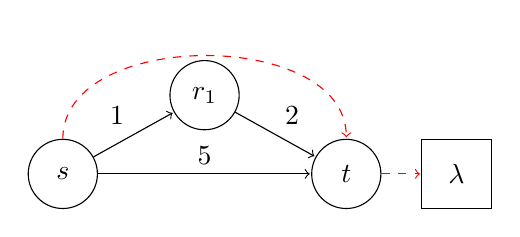
\begin{tikzpicture}[shorten >=0.5pt,node distance=,on grid,auto,
				square/.style={regular polygon,regular polygon sides=4}] 
				\node[state] at (0,0) (s)  {$s$}; 
				\node[state] at (1.8,1) (v1)  {$r_1$}; 
				\node[state] at (3.6, 0)(t) {$t$};
				\node[state, rectangle] at (5, 0) (d1) {$\lambda$};
				\path[->] 
				(s) edge node {1} (v1)
				edge  node {5} (t)
				edge [red, dashed, bend left=90] node {} (t)
				(v1) edge node {2} (t)
				(t) edge [red, dashed] node {} (d1);
				\end{tikzpicture}
			}}}
			\subfloat[Route-Filters]{
				\resizebox {0.5\columnwidth} {!} {
					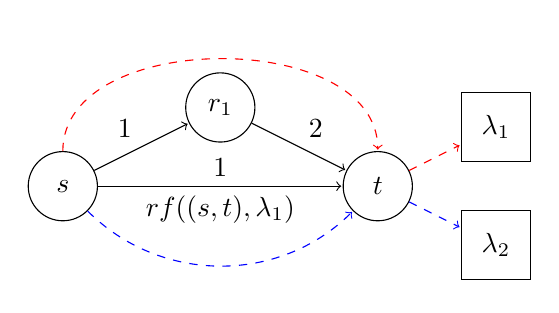
\begin{tikzpicture}[shorten >=0.5pt,node distance=,on grid,auto,
					square/.style={regular polygon,regular polygon sides=4}] 
					\node[state] at (0,0) (s)  {$s$}; 
					\node[state] at (2, 1) (v1)  {$r_1$}; 
					\node[state] at (4, 0)(t) {$t$};
					\node[state, rectangle] at (5.5, 0.75) (d1) {$\lambda_1$};
					\node[state, rectangle] at (5.5, -0.75) (d2) {$\lambda_2$};
					\path[->] 
					(s) edge node {1} (v1)
					edge  node [above] {1} node [below] {$rf((s,t),\lambda_1)$} (t)
					edge [red, dashed, bend left=90] node {} (t)
					edge [blue, dashed, bend right=45] node {} (t)
					(v1) edge node {2} (t)
					(t) edge [red, dashed] node {} (d1)
					(t) edge [blue, dashed] node {} (d2);
					\end{tikzpicture}
				}}
				\compactcaption{OSPF edge weights and filters such that the
					the routers forward traffic for destination along
					the input paths (dashed arcs).}
				\label{fig:ospfexample}
\end{figure}
			
\subsection{Simple OSPF Configurations} \label{sec:sarc}
 
For the OSPF protocol, configurations assign
 weights $W$ to links between routers (directed edges
 in the network topology);
 OSPF routers uses 
 Djikstra's algorithm to choose the
 shortest weighted path for a pair of endpoints. 
 Thus,
 given input paths, \name finds edge weights 
 (which are global for all paths) such that 
 the shortest path through the network
 for these endpoints exactly match the input paths. 
 For example in \Cref{fig:ospfexample}(a), if the input
 path is $s\rightarrow r_1 \rightarrow t$ for
 destination IP $\lambda$, \name assigns
 edge weights such that the input path has a strictly
 smaller weight ($W=1+2$) than the other path $s \rightarrow t$ 
 ($W=5$). Thus, the OSPF routers will forward traffic for
 $\lambda$ from $s$ to $t$ through $r_1$. We first
 consider the scenario of simple OSPF configurations (sOC)
 with no route-filters enabled.

The problem of synthesizing the
sOC that realizes an input set of paths reduces to a
variation of the so-called {\em inverse shortest path} 
problem~\cite{isp}. 
%Assume we are given the following inputs: (1) a directed graph $T = (S, L)$ (the network topology), 
%(2) a set of endpoints $\Gamma \subseteq S\times S$
%describing the sources and destinations of the input paths, and 
%(3) a function $P: \Gamma \rightarrow 2^{L^*}$
%that assigns to each pair of endpoints $(s,t) \in \Gamma$ 
%a set of \emph{acyclic} paths, such that for every path $l_0\cdots l_n\in P(s,t)$,
%$l_0=(s,s')$, for some $s'\in S$, and $l_n=(s'',t)$, for some $s''\in S$.\footnote{
%We use $L^*$ the denote the set of all finite sequences over $L$.}
%The 
%\emph{sARC synthesis}
%problem is to find rational weights for the edges in $L$ such that 
%for each pair of endpoints $(s,t) \in \Gamma$, 
%the paths in $P(s,t)$ are \emph{the} shortest paths from $s$ to $t$ 
%in the graph. Notice, that there can be multiple shortest
%paths of equal cost for multi-path support (e.g., for traffic engineering).
For a destination IP $\lambda$, we call $\xi_\lambda$ 
the directed tree of $T$ 
obtained by only keeping the nodes and edges 
that are traversed by paths in $\Pi$ for 
destination IP $\lambda$.
Since paths are acyclic, $\xi_d$ is a directed acyclic graph.
$\Delta=\{\xi_\lambda\mid \lambda \in \Lambda\}$ is   
the set of all destination trees. 

We use  $r_1\rightarrow r_2$ to denote $(r_1,r_2)\in L$ and
$r_1\rightarrow^* r_2$ (resp. $r_1\rightarrow^+ r_2$) to denote 
that $r_2$ is reachable from $r_1$ by crossing zero 
(resp. one) or more links in $T$.
Similarly, we use $\rightarrow_{\xi_\lambda}$ 
to denote the same relations in the destination trees.


\minisection{Distance equations}
To solve the sOC synthesis problem, 
we generate a set of linear equations
to find the edge weight $W(r_1, r_2)$ 
for all $(r_1, r_2) \in L$.
We use 
$D(r_1, r_2)$ to denote the 
shortest distance from $r_1$ to $r_2$.
We add the equation $D(s,s) = 0$ 
for every $s\in S$ to denote that the distance
from a node to itself is $0$.
The
following equation guarantees that $D(s,t)$ is not greater than 
the actual shortest distance from $s$ to $t$.
\begin{equation} \label{eq:dist}
\forall s, t. ~\forall r. ~r \in N(s).~
D(s, t) \leq W(s, r) + D(r, t)
\end{equation}

For each destination tree $\xi_d\in\Delta$, we add equations to ensure 
that the input paths with destination $d$ are indeed the shortest ones.
 If a path
is the shortest path between its endpoints, then every 
subpath of the path has to be the shortest between its endpoints
as well (otherwise the complete path would not be the shortest).

Consider a tree $\xi_d$ for destination $d$. We define two neighbour
functions: $N_T(s)$ denotes the set of neighbours of ritch $s$ 
in the input graph $T$, and $N_{\xi_d}(s)$ denote the set of
neighbours of ritch $s$ in the destination tree $\xi_d$. 
Given a destination $d\in \Omega$,
we use the following equations to ensure that, given two nodes $s$ and $t$ in
$\xi_d$, 
the set of paths from $s$ to $t$ in $\xi_d$ are
exactly
\emph{the} shortest paths from $s$ to $t$ in $T$.
Let $s$ and $t$ be two nodes in $\xi_d$ and let  $Paths_{\xi_d}(s,t)$ be the set of paths from $s$ to $t$ in $\xi_d$.
\begin{multline} \label{eq:uniq1}
		\forall l_0\cdots l_n\in Paths_{\xi_d}(s,t).
		\forall n' \in N(s) \setminus N_{\xi_d}(s). \\
		W(s, n') + D(n', t) > \sum_{\mathclap{\substack{l_i=(s_i,t_i)}}} 
		W(s_i, t_i) 
\end{multline}
\begin{multline} \label{eq:uniq2}
		\forall l_0\cdots l_n\in Paths_{\xi_d}(s,t).
		\forall n' \in N_{\xi_d}(s). n' \not\rightarrow^+_{\xi_d} t.  \\
		W(s, n') + D(n', t) > \sum_{\mathclap{\substack{l_i=(s_i,t_i)}}} 
		W(s_i, t_i) 
\end{multline}
\vspace{-2mm}
\begin{multline} \label{eq:uniq3}
		\forall l_0\cdots l_n, l_0'\cdots l_n'\in Paths_{\xi_d}(s,t).\\
		\sum_{\mathclap{\substack{l_i=(s_i,t_i)}}} 
		W(s_i, t_i)  =\sum_{\mathclap{\substack{l_i'=(s_i',t_i')}}} 
		W(s_i', t_i') 
\end{multline}
Equation~\ref{eq:uniq1} guarantees that 
the sum of the weights belonging to a path from $s$ to $t$ in $\xi_d$ is smaller than 
any path that goes to $t$ via a node $n'$ that is a neighbour of $s$ in $T$ but not in $\xi_d$.
Equation~\ref{eq:uniq2} guarantees that
the sum of the weights belonging to a path from $s$ to $t$ in $\xi_d$ is smaller than 
any path that goes to $t$ via a node $n'$ that is a neighbour of $s$ in $\xi_d$ but such that
$t$ is not reachable from $n'$ in $\xi_d$.
Finally, Equation~\ref{eq:uniq3} guarantees that all the paths from $s$ to $t$ in $\xi_d$ have the same weight.

\subsection{Synthesising Inter-domain Configurations}
\label{sec:inter-synthesis}


In this section, we present an algorithm for 
solving the path-compliance problem in the presence
of multiple domains---i.e., $|\{\Theta(r) \mid r\in V\}|>1$.
First, our algorithm determines the 
BGP configuration and static routes to ensure that the 
paths will traverse the correct domains.
Second, we show how to modify the 
techniques given in Section~\ref{sec:intra-synthesis}
to determine the edge weights and static routes
 in each domain to guarantee that paths traverse
the correct gateway routers.


\subsubsection{Configuring BGP and Static Routes}
BGP is a path-vector protocol where each BGP router,
for each destination $\lambda$,
advertises to its peers
what sequence of domains one should follow to get to  $\lambda$.  
In this section, we describe how to configure
BGP routers so that the routes chosen by BGP 
(and redistributed into OSPF) 
can yield the policy-compliant
paths $\Pi$ given as input. 
We need to take into account three different
cases, which are illustrated in \Cref{fig:bgpexample}.  
For sake of simplicity, we omit certain small details 
from the following discussion.

In the first case, a path is preferred because it traverses fewer domains.
For example, in \Cref{fig:bgpexample}(a), we want
path (1)---i.e., the red one---to be the chosen path from source $s$ 
to destination $\lambda$.
Here, BGP router $g_3$ receives from $g_6$ an advertisement for a route to destination $\lambda$
traversing only the domain $1$; this route has domain path length 1 as it only traverses 1 domain. 
Instead, $g_1$ and $g_2$ receive advertisements for a route 
(D2, D1)
to destination $\lambda$  with 
domain path length 2. Since our objective is to send traffic along
$g_3$, for path (1) we do not need to add any further BGP configurations,
and the route via $g_3$ is automatically redistributed into domain D0;
for destination $\lambda$, the gateway at domain D0 is $g_3$, i.e.,
$G^C(0, r_1, \lambda) = g_3$.

In the second case, the requested path does not have shortest domain path length
and we therefore need to set local preferences.
For example, let's say that in \Cref{fig:bgpexample}(a) we now want
path (2)---i.e., the purple one---to be the chosen path from source $s$
to destination $\lambda$. 
Since $g_1$'s route traverses more domains than
 $g_3$'s route,
we need to set the local preference of route received by $g_1$ 
(from $g_4$) to a value greater than the preference for the route received by $g_3$. 
In the example, we set the preference at node $g_1$: 
$LP(g_1, g_4, \lambda) = 100$
which causes $g_1$ to become gateway at domain D0 for destination $\lambda$, i.e., 
$G^C(0, r_1, \lambda) = g_1$.

In the third case, two paths from different sources in the same domain, but for the same destination $\lambda$, exit 
the domain through two different
gateways.
For example, in \Cref{fig:bgpexample}(b),
the path from $r_1$ to $\lambda$ exits domain D0 through 
gateway router $g_1$, while the path from $r_2$  to $\lambda$ exits 
through $g_2$. 
Moreover,  we assume that $g_1$ is the closest gateway to $r_1$ and 
$g_2$ is the closest gateway to $r_2$ w.r.t. OSPF paths in the domain.
In this case, both these routes need to be 
somehow redistributed to the OSPF domain. 
By assign local preferences such that
$LP(g_1,g_3,\lambda)<LP(g_2,g_4,\lambda)$,
we have that $g_2$ is advertised to the OSPF domain
and
the traffic from $r_2$ correctly exists through $g_2$. 
To prevent that the traffic from $r_1$ also exists through $g_2$,
we add an iBGP filter for the connection $g_2 \rightarrow g_1$ for
destination IP $\lambda$.\footnote{Gateways $g_1$ and $g_2$ need not be connected by a 
link directly; iBGP establishes a connection among the 
BGP routers in a domain.} Thus, $g_1$ will not receive the
$g_2 \rightarrow g_4$ route from $g_2$, 
and the route from  $r_1$ to $\lambda$ will exit through $g_1$.
%as it has the highest local preference
%of all routes received by $g_1$, and will be redistributed into the 
%OSPF domain. 
\begin{figure*}
	\centering
	\subfloat[Single
	BGP Gateway]{\includegraphics[width=0.305\columnwidth]{figures/bgp-example.pdf}}
	\hfill
	\subfloat[Multiple BGP Gateways]{\includegraphics[width=0.33\columnwidth]{figures/bgp-example2.pdf}}
	\hfill
	\subfloat[Static Routes]{\includegraphics[width=0.265\columnwidth]{figures/static-route.pdf}}
	\compactcaption{\label{fig:bgpexample}
		Examples of how BGP and static routes are configured for 
		inter-domain routing given a domain assignment $\Theta$.}
\end{figure*}

\minisection{Static Routes} \label{sec:static}
Next we describe a case in which standard BGP cannot enforce
the desired path, therefore requiring the use of static routes.
Consider the path for destination $\lambda$ 
shown in \Cref{fig:bgpexample}(c). BGP Gateway $g_1$, which is in
domain D0, 
will receive an advertisement for $\lambda$ that goes through domain
1 and then domain D0.
This advertisement will be rejected because it creates a loop---i.e., the domain D0
appears twice in the path. 
To enforce domain paths with loops, we use static routes. In this example
the static routes
$SR(r_1,\lambda) = r_2$, $SR(r_2,\lambda) = g_1$, and $SR(g_1,\lambda) = g_2$ 
guarantee that routes from $r_1$, $r_2$, and $g_2$ to $\lambda$ traverse the desired links.
Notice that the path from $g_2$ to $\lambda$ does not 
require static routes, as there are no domain loops.

\minisection{Algorithm}
We are now ready to describe the algorithm that,
given a set of paths $\Pi$, determines
BGP local preferences, iBGP filters, and static routes for enforcing such paths.
For a path $\pi = l_1 l_2 \ldots l_m \in \Pi$, we
can divide the path into intra-domain paths and inter-domain
links. We express $\pi$ as 
$\pi_1 idl_1^2 \pi_2 \ldots idl_{n-1}^n \pi_n$ where
each subpath $\pi_i$ is completely in a
domain, i.e., for each 
link $(r_1,r_2) \in \pi_i \implies \Theta(r_1) = \Theta(r_2)$;
and links $idl_1^2, idl_2^3 \ldots idl_{n-1}^n$ 
represent the inter-domain links, i.e., 
if $idl_i^{i+1}=(r,r')$ then $\Theta(r_1) \neq \Theta(r_2)$. 
The domain path
$\tilde{\pi} = d_1 \ldots d_n=\Theta(\pi_1)\ldots \Theta(\pi_n)$ describes the 
domains traversed by $\pi$ (where
$\Theta(\pi_i)$ denotes the domain of the routers in the 
domain path $\pi_i$). 


For a given path $\pi$ and corresponding path $\tilde{\pi}$,
we find the longest non-looped domain subpath ending in domain
$d_n$. Formally, we find the smallest index $nl$ such that
$\forall j \geq nl. ~\neg\exists k \geq i.~d_j = d_k$. 
The loop-free subpath $\pi'=\pi_{nl} ~idl_{nl}^{nl+1}\ldots idl_{n-1}^n \pi_n$ corresponding to
domains $d_{nl} \ldots d_n$
can be induced using BGP, as described in \Cref{fig:bgpexample}(a)
and \Cref{fig:bgpexample}(b).
For all links that are not in $\pi'$
we will require static routes.
With abuse of notation, for every link $(r_1,r_2)\in\bigcup_{i< nl} \pi_i\cup \bigcup_{i< nl}\{l_i^{i+1}\}$ 
we have
$SR(r_1, \lambda) = r_2$.

Finally, for each intra-domain subpath $\pi_i$ that is not statically routed---i.e., $i\geq nl$---\name applies
OSPF synthesis for the domain $\Theta(\pi_i)$. 
This is done after aggregating by domain across all subpaths obtained when processing all paths in $\Pi$.
We describe this in the next section.
%For each destination $\lambda \in \Lambda$, 
%BGP is configured accordingly
%based on if there is a single gateway in domain (\Cref{fig:bgpexample}(a))
%or multiple gateways (\Cref{fig:bgpexample}(b)) for the paths of destination
%$\lambda$ in the domain. 



%Static routes have the highest priority and is used to 
%exit and enter a domain multiple times. 
%While static routes
%do not reduce the resilience of the network (all routes are still
%enabled, unlike route filters), a network under flux will have
%unpredictable routing behaviour, unlike with only OSPF and BGP
%configured at the routers. 
%Also, static routes have to be installed per-destination, thus increasing
%the size of configurations drastically as number of policy paths increase.
%
%Given a path $p$ for subnet $\lambda$ and 
%the corresponding domain path $p_{as}
%= as_1 \rightarrow as_2 \rightarrow \ldots \rightarrow as_m$ (where
%$as_m = \Theta(\lambda)$), static
%routes are required if $p_{as}$ has a domain-loop. 
%To minimize
%the number of static routes, we find 
%the smallest $i \in [1,m]$ 
%such that $\overline{p_{as}} = as_i \rightarrow as_{i+1}
%\rightarrow \ldots \rightarrow as_m$ has no loops. 
%Therefore, $\overline{p_{as}}$ is the longest domain-loop-free
%subpath of $p_{as}$, and be can be enforced using BGP and OSPF. For the 
%network path corresponding to domain path $as_1 \rightarrow as_2 
%\rightarrow \ldots \rightarrow as_{i-1}$, we require static
%routing rules for each next-hop. The static routing score
%is the total number of static route hops required to enforce
%the input paths.
%\todo{Write about the BGP paths are extracted for the next phase}
%
%\subsubsection{BGP Local Preference Entries}
%\name uses BGP local preference to route traffic
%for a particular subnet to the next domain via a specific 
%gateway as per the input paths obtained. 
%As shown in \Cref{} (Refer
%to ex), if there are multiple exit gateways from an domain 
%for a subnet $\lambda$, we require local preference entries at the 
%gateways and iBGP filters among these gateways for $\lambda$.
%
%For a domain $d$ and subnet $\lambda$, consider the set 
%of paths to $\lambda$ exiting $d$ using BGP (and not statically
%routed as described in \Cref{sec:static}). Let $E$ denote the
%set of exit gateway routers for the paths of $\lambda$. 
%If $|E| = 1$, if gateway $g$ receives a route with 
%strictly shortest domain path length (\Cref{alg:bgppathrules}) 
%which enforces the paths
%for $\lambda$, we do not need to configure local preference
%entries on any BGP router in the domain for $\lambda$. If
%the exit route chosen by the gateways for $\lambda$ does not 
%enforce the paths, \name configures a local preference entry
%for $\lambda$ at exit gateway, and thus, the exit route chosen
%by BGP enforces the input paths for $\lambda$ in the domain.
%
%If $|E| ~> 1$, multiple BGP routes must be redistributed to 
%the OSPF domain.
%E local prefs + E(E - 1) iBGP filters!
%
%\todo{Changes to OSPF synthesis to ensure closest gateway}
\subsubsection{Modified OSPF Synthesis for Multiple Gateways}
When BGP routes for destination $\lambda$ 
are redistributed by multiple gateways to an 
OSPF domain, \name uses a modified OSPF synthesis
algorithm from \secref{sec:intra-synthesis} to assign OSPF weights to the links in each domain
and place static routes. 
This is 
required because an OSPF router will choose
the closest BGP gateway in terms of OSPF distance 
for $\lambda$. For instance, a router $r$ will choose
from gateways $g_1$ over $g_2$ if the OSPF distance from $r$ to $g_1$ 
is strictly lesser than the distance from $r$ to $g_2$. 
Assume we are given the input subpath $\pi_i=r \rightarrow^+ g_1$ in
the domain $d=\Theta(\pi_i)$ for some destination $\lambda$ outside
of $d$; this path should exit through gateway $g_1$. 
\name adds additional
constraints ensuring the distance to $g_2$ from routers
on the path $\pi_i$ is strictly
greater than the distance to $g_1$. 

Let $G(\theta, \lambda)$ be the set of gateway
routers for destination $\lambda$ in a given domain $\theta$. 
We define the relation $r_1 \rightarrow^+_{\xi_{\lambda}} r_2$, which holds if
$r_2$ is reachable from $r_1$ in the destination tree $\xi_\lambda$.
For each subpath $r \rightarrow^+_{\xi_{\lambda}} g$ to destination $\lambda$
and for each $g' \in G(\theta, \lambda)$ such that $g\neq g'$,
\name adds the following constraint
to ensure that the  router $r$
chooses the correct gateway: 
\begin{equation} \label{eq:gateway}
\forall r' \in N(r) \setminus N_{\xi_\lambda}(r).~
\sum_{\mathclap{\substack{(r_1,r_2) \in r \rightarrow^+_{\xi_{\lambda}} g }}}~~~~~W_{r_1}^{r_2} < 
W_r^{r'} + D_{r'}^{g'} 
\end{equation}
If the system of
constraints generated is inconsistent, Zeppelin will add 
static routes to eliminate constraints
and filter shorter routes to gateways which are
not on the input path. For Equation~\ref{eq:gateway},
adding the static route $(r, N_{\xi_\lambda})$ to $SR(\lambda)$
will eliminate the infeasibility caused due to this equation.

\section{Waypoint-Compliance Synthesis}
Middleboxes like firewalls,
proxies, intrusion detection and prevention systems and 
optimizers play a crucial role in enterprise and
datacenter networks for security, performance 
and auditing considerations. Enforcing waypoint policies for
middlebox traversals is one of the most common policies 
supported by network operators. When a 
tenant specifies a waypoint policy, 
for e.g., traffic from
subnet A to subnet B must traverse 
through a firewall, the control plane need not
route traffic through a particular path, but ensure
that the path through the network traverses the firewall. 
Thus, instead of enforcing the path provided by \genesis,
we extend \name to provide support for \emph{waypoint-compliance}
synthesis (\secref{sec:ospfwaypoint}). 

Another matter of consideration for tenants is 
policy-compliance under failures (which are frequent in 
datacenter networks), which can violate key security 
properties. For example, 
traffic for a particular subnet under 
failure scenarios can become vulnerable to attacks if the 
path in the network no longer traverses the firewall. 
However, providing compliance 
guarantees for all policies
under arbitary link failures is a difficult problem, 
especially in a traditional control plane 
which reacts to failures in a distributed fashion. 

\name incorporates policy-compliance
for a subset of waypoint policies 
under bounded link failure scenarios without the 
need for intervention by a central controller by 
leveraging the emerging field of NFV. 
Network Function Virtualization (NFV) has been a 
major driving force for providing reliability 
guarantees under failures  
for middlebox traversals~\cite{opennf, netbricks}. 
Using NFV technology, operators can replicate 
their middleboxes across the network for providing 
resilience guarantees. For waypoint policy-compliance, 
we define a \emph{waypoint set} 
which denotes the set of physical replicas of the 
middlebox and ensure that routing under a bounded 
number of failures traverses an element in the waypoint
set. In this paper, we will describe the approach to  
provide resilience guarantees for arbitary single
link failures (\secref{sec:ospfresilience}).


\subsection{Problem Statement}
Let us consider an 
unordered waypoint policy of the form: 
\texttt{$\lambda$: s >> \{$W_1$, \ldots $W_n$\} >> t},
where $\lambda$ is the destination IP subnet,  
$s$ and $t$ are the source and destination router respectively, 
and $W_1, W_2 \ldots W_n \subseteq V$ are waypoint sets. This
policy is mapped to a packet class $pc \in \nat$. A path 
$\pi$ is policy-compliant iff the path from $s$ to $t$ traverses
through a waypoint $w_i \in W_i$ for all $i=\{1,\ldots n\}$. 
The configuration $C$ is waypoint-compliant for packet class $pc$ 
iff: 
\[
\exists \pi \in \paths^C(pc). ~\forall i \leq n. ~\exists w_i \in W_i. 
~\exists u. ~~(u, w_i) \in \pi 
\]
where $\paths^C(pc)$ is the set of induced paths for 
$pc$ by configuration $C$ (Definition~\ref{def:inducedpaths}). 

A configuration $C=(T,\Theta,W,LP,IF,SR)$ is 1-resilient 
for packet class $pc$  
iff for all 
$T' = (V, L'), |L'| = |L| - 1$, the configuration $C'
=(T',\Theta,W,LP,IF,SR)$  
is waypoint-compliant for packet class $pc$. 

\definecolor{orange}{RGB}{255, 157, 30} 
\begin{figure}[!t] 
	\centering
	\subfloat[Edge Weights]{
		\resizebox {0.33\columnwidth} {!} {
				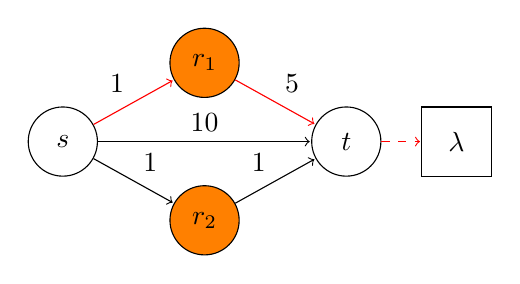
\begin{tikzpicture}[shorten >=0.5pt,node distance=,on grid,auto,
				square/.style={regular polygon,regular polygon sides=4}] 
				\node[state] at (0,0) (s)  {$s$}; 
				\node[state, fill=orange] at (1.8,1) (v1)  {$r_1$}; 
				\node[state, fill=orange] at (1.8,-1) (v2)  {$r_2$}; 
				\node[state] at (3.6, 0)(t) {$t$};
				\node[state, rectangle] at (5, 0) (d1) {$\lambda$};
				\path[->] 
				(s) edge [red] node [black] {1} (v1)
				(s) edge  node {1} (v2)
				edge  node [above] {10} (t)
				(v1) edge [red] node [black] {5} (t)
				(v2) edge  node [black] {1} (t)
				(t) edge [red, dashed] node {} (d1);
				\end{tikzpicture}
			}}
		\subfloat[Routing Loop]{
\raisebox{0.7cm}{\resizebox {0.33\columnwidth} {!} {
	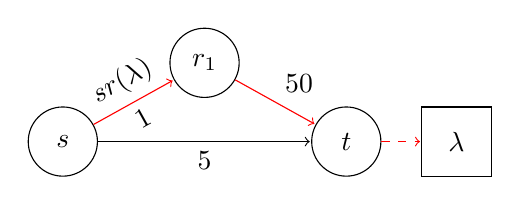
\begin{tikzpicture}[shorten >=0.5pt,node distance=,on grid,auto,
	square/.style={regular polygon,regular polygon sides=4}] 
	\node[state] at (0,0) (s)  {$s$}; 
	\node[state] at (1.8,1) (v1)  {$r_1$}; 
	\node[state] at (3.6, 0)(t) {$t$};
	\node[state, rectangle] at (5, 0) (d1) {$\lambda$};
	\path[->] 
	(s) edge [red] node [black, sloped, anchor=center, above]
	{$sr(\lambda)$} node
	[black, sloped, anchor=center, below] {1} (v1)
	edge  node [below] {5} (t)
	(v1) edge [red] node [black] {50} (t)
	(t) edge [red, dashed] node {} (d1);
	\end{tikzpicture}
}}}
	\compactcaption{OSPF edge weights such that the path is waypoint-compliant and example of routing loop created by a static route.}
	\label{fig:ospfw}
\end{figure}
\subsection{Intra-domain Waypoint Compliance}\label{sec:ospfwaypoint}
Let us consider a waypoint policy for $\lambda$ which
specifies that traffic to $\lambda$ must traverse through
one of the waypoints $w \in \waypt$, where $\waypt \subseteq V$.
In the first phase, \genesis provides a path which
satisfies the waypoint policy. We use this path as a 
``hint'' to incorporate waypoint-compliance in the OSPF 
configuration synthesis without 
enforcing the exact path.

We define $D_s^t(\waypt)$ to be the 
distance between $s$ and $t$ such that the path does not
 traverse through any waypoint $w \in \waypt$. Intuitively, we
  can add constraints to represent these distances by
  considering a network topology where all the  
  waypoints $w \in \waypt$ are removed. Formally, for a topology 
 $T = (V,L)$, the following distance equations 
 capture the non-waypoint distances 
 for a waypoint set $\waypt$:
\begin{equation} \label{eq:wdistance}
\forall s, t \in V \setminus \waypt. ~\forall r \in N(s) \setminus \waypt.~
D_s^t(\waypt) \leq W_s^r + D_r^t(\waypt)
\end{equation}
These constraints are similar to the constraints specified in
\Cref{eq:distance}, but for an ``altered'' topology where all
the waypoint routers are removed, and thus, any path in this 
topology is not compliant with the waypoint policy. 
Similar to $D_s^t$ variables, 
$D_s^t(\waypt)$ is upper bounded by the actual shortest non-waypoint distance from $s$ to $t$.

Given a destination tree $\xi_\lambda$, we will use the 
non-waypoint distances to enforce waypoint-compliance. Consider a 
router in $r$ such the waypoint $w \in \waypt$ is downstream to $r$ in $\xi_\lambda$
(there exists a path from $r$ to $w$ in $\xi_\lambda$), therefore,
the path from $r$ must traverse through 
a waypoint in $\waypt$.  
Suppose, the sum of weights of the edges of
the path in the tree $W(r \rightarrow^+_{\xi_\lambda} R_\lambda)$  
is strictly smaller than the non-waypoint 
distance from $r$ to $R_\lambda$. This will ensure that 
the shortest path from $r$ to $R_\lambda$ which does not go through
any $w \in \waypt$ will have a distance strictly greater than the path through
$\xi_\lambda$, thus, the path from $r$ to $R_\lambda$ will traverse
through a waypoint $w \in \waypt$. These constraints are expressed as follows:
\begin{equation} \label{eq:waypoint}
\forall r' \in N(s) \setminus N_{\xi_\lambda}(r).~~ \sum_{\mathclap{\substack{l_i=(r_1,r_2)}}} 
W_{r_1}^{r_2} < 
W_{r}^{r'}+ D_{r'}^{R_\lambda}(\waypt) 
\end{equation}
Note that, unlike Equations~\ref{eq:unique}, in this case, 
router $r$ will not necessarily forward traffic to  
$N_{\xi_\lambda}(r)$, but the path chosen will be waypoint-compliant. 
Consider the example in \Cref{fig:ospfw}(a) where traffic for
$\lambda$ must traverse through one of the waypoints $\{r_1, r_2\}$. 
Observe that while \genesis provided the path $s \rightarrow 
r_1 \rightarrow t$, in the solution provided by Zeppelin, 
the shortest path is $s \rightarrow r_2
\rightarrow t$, and both waypoint-compliant paths are shorter 
than $s \rightarrow t$, the shortest non-waypoint path.

If one of these constraints was part of an unsatisfiable  
core, we can add the static route $(r, N_{\xi_\lambda}(r))$ to
$SR(\lambda)$ to eliminate the equations at router $r$. 

\minisection{Routing Loop Avoidance Constraints} \label{sec:loopavoidance}
Since we are not enforcing a particular path in the network for waypoint-
compliance, adding
static routes can lead to undesired behaviors like routing loops.  
Consider the example configuration shown in \Cref{fig:ospfw}(b). 
Traffic for $\lambda$ at router $s$ is forwarded to $r_1$ because of the
static route at $s$. At router $r_1$, the shortest OSPF route to
$\lambda$ is $r_1 \rightarrow s \rightarrow t$ with weight 6 (compared 
to $r_1 \rightarrow t$ of weight 50). Thus, $r_1$ will send the 
packet back to $s$, and thus, causing a routing loop as $s$ will send
it back to $r_1$ and back and forth till the \emph{ttl} (time to live) of the
packet expires. 

Zeppelin adds additional constraints to mitigate the creation of prevention
of routing loops when static routes are added. In each iteration of
Zeppelin's unsat-core learning procedure: 
Zeppelin picks a static route $(r, r')$
for $\lambda$ and removes the constraints pertaining to 
the static route. It also \emph{adds} new constraints to avoid
causing routing loops due to the newly added static route. This
lazy approach ensures we do not add superflous constraints for links
that do not contain a static route in the final configuration 
and will not cause routing loops. \name does not sacrifice 
soundness by lazily adding the loop avoidance constraints. 

Suppose, Zeppelin added a static route $(sr_1, sr_2)$ for destination
$\lambda$ where $sr_2 = N_{\xi_\lambda}(sr_1)$ (because we do not add
static routes on any other links except $\xi_\lambda$). We need to
ensure that for any router in $\xi_\lambda$ which does not 
lie in the downstream path $sr_2 \rightarrow^+_{\xi_\lambda} R_\lambda$, 
the shortest path from $sr_2$ to $R_\lambda$ must not traverse through 
it, for that could potentially cause a routing loop. For example, in \Cref{fig:ospfexample}(c), the shortest path from $r_1$ to $t$ was
going through $s$ (which is upstream of $r_1$), therefore, causing 
a routing loop. 

Therefore, to prevent routing loops, we ensure that the weight
of path $W(sr_2 \rightarrow^+_{\xi_\lambda} R_\lambda)$ is 
strictly smaller than any path from $sr_2$ which traverses a
router $r'$ not in the downstream path from $sr_2$. Zeppelin
adds the following constraints to ensure that the path $l_0...l_k$
from $sr_2$ to $R_\lambda$ is shorter than the paths which reach 
$R_\lambda$ through $r'$: 
\begin{equation}
\forall r' \in \xi_\lambda. ~sr_2 \not\rightarrow_{\xi_\lambda}^+ r'. 
~~~~~\sum_{\mathclap{\substack{l_i=(r_1,r_2)}}} 
W_{r_1}^{r_2} < D^{r'}_{sr_2} + D_{r'}^{R_\lambda} 
\end{equation}
If one of these constraints is part of an unsatisfiable
core, we need to add a static route to eliminate the 
unsatisfiability. When the constraint is part of the 
unsatisfiable core, it means that there is a routing 
loop caused at $sr_2$. By adding a static route 
$(sr_2, N_{\xi_\lambda}(sr_2))$ to $SR(\lambda)$, we prevent
the occurence of the routing loop from $sr_2$ and thus, can
remove these constraints. After we add the static route,
we add loop avoidance constraints for the new static
route, and continue with the unsat-core learning algorithm. 

\subsection{Intra-domain Resilience} \label{sec:ospfresilience}
Let us consider a waypoint policy for $\lambda$ which
specifies that traffic to $\lambda$ from router $s$ 
must traverse through
one of the waypoints $w \in \waypt$. We assume that 
all the waypoints belong in the same domain, i.e., 
$|\{\Theta(w) | w \in W\}| = 1$. NFV provides 
flexibility of waypoint placement in the network, 
and we can ensure
all replicas belong to the same domain.  
Suppose the tenant 
specifies that under any single link failure, the traffic 
to $\lambda$ must be waypoint-compliant; this is defined 
as \emph{1-resilient waypoint-compliance}. The constraints 
described in \secref{sec:ospfwaypoint} ensure waypoint-compliance
only when all links are functional, compliance is uncertain
when a link fails. We now discuss the approach of incorporating
resilience in the intra-domain configuration synthesis.

Instead of just adding constraints which ensure that a single 
waypoint-compliant path (provided by Genesis) is strictly 
shorter than the non-waypoint distance, we can leverage \genesis's
support for isolation to generate two edge-disjoint\footnote
{The edge-disjoint paths will actually be vertex-disjoint (except the 
	source and destination) due to the destination-tree constraints
	in \genesis.} paths
which are waypoint-compliant with respect to $\waypt$. A single link
failure will not disable both these paths, so if traffic to $\lambda$ 
would 
traverse one of these two paths under failures, 
we would achieve 1-resilient
waypoint-compliance. 

Assume that the OSPF domain does not allow any static routes. 
We use Genesis to provide two waypoint-compliant 
edge-disjoint paths $\pi_1$ amd $\pi_2$ from $s$ to $t$.
Equations~\ref{eq:waypoint} ensure that the edge weights 
of the path provided by Genesis are strictly shorter than 
the non-waypoint distance for $\lambda$. By adding these
constraints for both paths $\pi_1$ and $\pi_2$ provided by Genesis,
we enforce a \emph{partial order}: there are two paths to $\lambda$
which are shorter than non waypoint distance, the 
ordering of the weight of $\pi_1$ and $\pi_2$ is irrelevant. 
\begin{equation} \label{eq:resilience}
\{ W(\pi_1), W(\pi_2) \} < D^t_s(\waypt) 
\end{equation}
Thus, if a single link fails, only of these paths is affected. Suppose
$\pi_1$ is affected, OSPF will not route traffic a  
non-waypoint-compliant path, as the weight of $\pi_2$ is shorter than any path which is not waypoint-compliant due to the constraints generated 
by \name.

\minisection{Resilience with Static Routes}
Let us consider the case when there are static routes in the OSPF
domain. This complicates the synthesis of resilient configurations. 
Consider $\pi_1$ and $\pi_2$ are two edge disjoint paths 
connecting the routers $s$ to $t$. Suppose, $\pi_1$ is the 
chosen primary path and it uses static routes on 
some of its links.
Ideally, we want to ensure 
that if any link on $\pi_1$ fails, 
then the network must switch over to $\pi_2$. 

A static route $(r_1, r_2)$ on path $\pi$ for destination $\lambda$ implies that OSPF routing at $r_1$ is sending traffic to a 
router $r' \not= r_2$ and the OSPF path would be violating
waypoint-compliance. Instead, the static route circumvents 
the OSPF shortest route at $r_1$ and \emph{steers} $\lambda$ 
traffic to $r_2$ and not $r'$. Therefore, for a 
path $\pi$ connecting routers $s$ and $t$ such that it 
has a static route on one of its links, 
then $W(\pi)$ is greater than or equal to the 
actual OSPF distance
between $s$ and $t$ (which is the OSPF route at $s$).
Let us suppose $\pi = l_1 \ldots l_k = (u_1, v_1) \ldots (u_k, v_k)$ 
and 
there exists a $\alpha \leq k$ such that 
$l_\alpha = (u_\alpha, v_\alpha)$  
is the first 
static route from the source in $\pi$, i.e., 
$\forall 1 \leq \beta < \alpha. ~(u_\beta, v_\beta) \not\in SR(\lambda)$.
Therefore, all routers between $s$ and $u_\alpha$ did
not require any static routes to steer traffic along a 
non-shortest path. Therefore, we can estimate the 
actual shortest OSPF distance between $s$ to $t$ as:
\[
\sum_{i=1}^{\alpha - 1} W_{u_i}^{v_i} + D_{u_\alpha}^t
\]


Coming back to the synthesis of resilient configurations,
when \name adds static routes for \emph{steering},  
the partial order \Cref{eq:resilience} is not necessarily true 
(the partial order would hold only under no failures and 
no static routes). 
Because of that, when the primary path $\pi_1$ fails, the 
failover path $\pi_2$ may not be chosen. To ensure that 
$\pi_2$ is always chosen, we try to split the traffic
along $\pi_1$ and $\pi_2$, therefore, a failure to $\pi_1$
will still ensure that traffic is sent through $\pi_2$ 
(which is waypoint-compliant). To enforce splitting amongst
$\pi_1$ and $\pi_2$, we add the following constraints: 
\begin{equation}
	W(\pi_2) \leq \sum_{i=1}^{\alpha - 1} W_{u_i}^{v_i} + D_{u_\alpha}^t	
\end{equation}
where $(u_\alpha, v_\alpha)$ is the first static route in $\pi_1$.
We add symmetric constraints constraining $W(\pi_1)$. 

Similar to the routing loop avoidance constraints, we add the
above constraints lazily when a static route is added to one of the
paths for $\lambda$. However, if one of these constraints is part of 
an unsatisfiable core, we cannot add a static route to eliminate 
this unsatisfiability. \name lazily eliminates these constraints from the
system of equations depending on whether these constraints are part of 
an unsat-core which cannot be eliminated by a static route. Thus, 
our resilience synthesis is not sound and for certain failure scenarios, 
the paths generated are not waypoint-compliant. However, 
based on our experiments (\secref{sec:reseval}), 
this technique generates highly resilient configurations 
in practice. 


\section{Synthesising Domain Assignments}
\label{sec:synth-dom-ass}
Many networks today have well-defined routing hierarchies to realize a variety of administrative  policies or division of responsibilities. For example, a campus network may be hierarchically divided into multiple routing domains (e.g., OSPF Areas) corresponding to different departments. Often, these hierarchies are realized through careful planning, and require detailed configurations, e.g., to determine which routers to include in a particular OSPF routing domains, how many such domains to create, how big to make each domain etc. Unfortunately, this makes the hierarchical division painstaking and error-prone, but also the careful planning means that changes to the hierarchies, e.g., to accommodate more hosts or new policies, are difficult to implement.

In such settings, Zeppelin can help by automating domain creation/restructuring. It can automatically find good routing domain hierarchies with increased resilience/decreased complexity and policy compliance. We envision that operators will synthesize “one-shot” domain assignments for their changing input policies at coarse-grained timescales (days/weeks) when there are significant changes to their networks or policies; operators need not resynthesize these assignments for every low-level policy change.


In this section, we present an algorithm for 
solving the path-compliance synthesis problem when a domain assignment is not given to us (Definition~\ref{def:pathcompliance}).
The algorithm searches the space of possible domain assignment $\Theta$ to find
one that meets all configuration policies and has good quantitative properties---e.g., minimizes
the number of static routes. 
%Formally, we are given 
%a topology $T=(V,L)$, a set of paths $\Pi$ and
%configuration policies $P$, 
%we want to find functions
%$W,RF,LP,IF,SR$ and $\Theta$ such that
%$C=(\Theta,W,$ $RF,LP$,$IF,SR)$,
%$C$
%We call this problem the \emph{domain assignment problem}.
%
We first show that when the domain assignment is not given,
even the simplest variant of the path-compliance assignment problem
is computationally hard.
\begin{theorem}
If $P$ disallows the use of static routes ($sc \leq 0$)
the path-compliance synthesis problem is NP-complete.
\end{theorem}
\iffull
%!TEX root = paper.tex
\begin{proof}
We show the $k$-graph coloring problem, which is NP-complete
reduces to finding a domain assignment such that the number
of static routes is 0. 
The latter is also in NP, so after the reduction we 
can conclude that it is also NP-complete.

Let $G = (V,E)$ be an instance of the 
$k$-graph coloring problem. Formally, 
we need to find a coloring $C: V \mapsto \{1,2,\ldots k\}$
such that for $\forall (u, v) \in E. C(u) 
\not= C(v)$.

\begin{figure}[H]
	\centering
	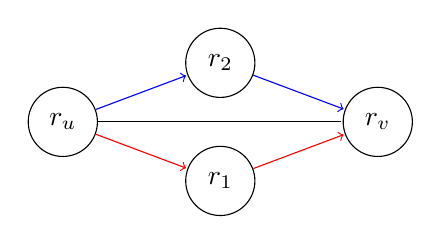
\begin{tikzpicture}[shorten >=0.5pt,node distance=1.5cm,on grid,auto,
	square/.style={regular polygon,regular polygon sides=4}] 
	\node[state] at (0,0) (s)  {$r_u$}; 
	\node[state] at (2,-0.75) (v1)  {$r_1$}; 
	\node[state] at (2,0.75) (u1)  {$r_2$};
	\node[state] at (4,0) (t) {$r_v$};
	\path[->] 
	(s) edge [red] node {} (v1)
	edge  [blue]  node {} (u1)
	(u1) edge [blue] node {} (t)
	(v1) edge [red] node {} (t);
	\path[-] 
	(s) edge node {} (t);
	\end{tikzpicture}
	\caption{Construction for reduction to Graph Coloring.}
	\label{fig:domasscomplexity}
\end{figure}

\paragraph{Construction.}
Let us consider a network topology $T = (R,L)$. 
For each $v \in V$, add a router $r_v \in R$. To
ensure any domain assignment to the $r_v$'s is valid, we 
add link to connect every router (each domain must be 
contiguous).

For every edge $(u, v) \in E$, we add $r_1, r_2$ to R, and add
paths: $r_u \rightarrow r_1 \rightarrow r_v$ and 
 $r_u \rightarrow r_2 \rightarrow r_v$ with different destinations
 to $\Pi$. We can notice that these two paths form a diamond. 
 
Suppose we find a domain assignment $\Theta$ 
with $k$ domains such that the number of 
static routes used is zero. 
Since, the count of static routes is 0, 
for two routers $r_u, r_v$ which 
have a diamond, $\Theta(r_u) \not= \Theta(r_v)$. This is
because, if $\Theta(r_u) = \Theta(r_v)$, then atleast 
one static route would be required to eliminate the diamond (Lemma~\ref{lemma:diamond}). 
Therefore, for every edge in $(u,v) \in E$, 
the routers $r_u$ and $r_v$ belong to 
different domains, therefore $u$ and $v$ have different colors. 
There, the $k$-graph coloring problem reduces to finding 
a domain assignment with zero static routes.  
Therefore, the policy-compliance synthesis problem is NP-complete.
\end{proof}




\fi

Given the complexity of this problem, we opt for a greedy
stochastic search.
\name searches the space of assignments using Markov
Chain Monte Carlo (MCMC) sampling methods, specifically the Metropolis-Hasting
algorithm, a common technique used in several optimization 
problems~\cite{stoke}. 
We first present the general structure of our search 
algorithm and 
then describe how the quantities 
in Table~\ref{tab:configpolicysupport} can be computed
or estimated to drive the search.



\subsection{Searching Assignments with MCMC}
MCMC sampling is a technique for 
drawing elements from a
probability density function in direct proportion to its value.
In our setting, MCMC searches the space of domain assignments and,
if we assign higher probabilities to domain assignments with lower cost, MCMC will explore
good configurations more \emph{often} than bad ones.
For MCMC to work we need to provide a transition function that lets us move from one domain assignment
to another with a certain probability and a cost function that assigns costs (and therefore probabilities) to
domain assignments. 

In our setting, each domain assignment $\Theta$
has an associated cost $c(\Theta, e)$
where
$e=expr(rc, sc, bc)$
is the expression we are trying to minimize---e.g., if we are trying to minimize the number of static routes $e=sc$.
We will discuss how our cost function is implemented in the Section~\ref{sec:cost-fun}.
%Given the cost function $c(.)$ and probability density 
%function $p(.)$, 
%the Metropolis acceptance probability~\cite{metropolis}
%for a transition from $\Theta \rightarrow \Theta'$ is as follows:
%\begin{multline}
%Pr(\Theta \rightarrow \Theta') = min(1, \frac{p(\Theta')}{p(\Theta)}) \\
%= min(1, exp(-\beta.(C(\Theta') - C(\Theta)))
%\end{multline}
%where $\beta$ is a positive constant. With the Metropolis
%algorithm, we can perform MCMC without calculating the actual
%probability density function $p(.)$, the arbitary cost function $c(.)$
%will suffice.

The search starts by setting the current domain assignment 
to some random domain $\Theta_0$.
The following process then repeats.
Given the current domain
assignment $\Theta$, 
compute a new domain assignment $\Theta'$ by randomly
moving a gateway 
router $r$ from one domain to another---i.e., $\Theta(r){\neq}\Theta'(r)$ and
for every $r'{\neq} r$, $\Theta(r'){=}\Theta'(r')$.
If $c(\Theta',e)\leq c(\Theta,e)$, then $\Theta'$ becomes the current domain assignment.
If $c(\Theta',e)>c(\Theta,e)$, then $\Theta'$ becomes the current domain assignment
with probability $Pr(\Theta \rightarrow \Theta')= exp(-\beta\times(c(\Theta',e) - c(\Theta,e))$ (where $\beta$ is a positive constant) 
while 
 $\Theta$ continues being the current domain assignment with probability $1-Pr(\Theta \rightarrow \Theta')$.
\iffull
The procedure is illustrated in \Cref{alg:mcmc}.
\fi

The algorithm always accepts a new proposal $\Theta'$
that has cost lower than $\Theta$. If $\Theta'$ has a 
higher cost than $\Theta$, the proposal is
accepted with probability inversely proportional to
how far the costs of $\Theta$ and $\Theta'$ are. This ensures that 
the algorithm does not get stuck at local minima, but 
explores proposals with small cost differences with 
higher probability.

\iffull
\begin{algorithm}[t]
	\floatname{algorithm}{Algorithm}
	\caption{Markov Chain Monte Carlo search for  finding a
	domain assignment that minimizes the expression $e$}
	\label{dcsyn}
	\begin{algorithmic}[1] \label{alg:mcmc}
		\Procedure{MCMCSearch}{$e$}
		\State{$\Theta \leftarrow$ random domain assignment}
%		\State{$\overline{cc} = 0$ \hspace{2cm} [Worst Conf. overhead]}
%		\State{$\overline{rc} = 0$ \hspace{2cm} [Worst route filter est.]}
		\While{max iterations OR timeout}
		\State{$\gamma$ = \Call{Cost}{$\Theta, e$}}
		\State{$\Theta'$ = \Call{RandomChange}{$\Theta$}}
		\State{$\gamma'$ = \Call{Cost}{$\Theta, e$}}
%		\State{$Pr(\Theta \rightarrow \Theta')$ = 
%			min$(1, exp(-\beta.(\gamma' - \gamma))$}
		\State{Set $\Theta$ = $\Theta'$ with 
			probability $Pr(\Theta \rightarrow \Theta')$}
		\EndWhile
		\EndProcedure
		
%		\Procedure{Cost}{$\Theta$} 
%		\State{$cc \leftarrow$ Configuration overhead (Static routes + \newline \hspace*{1.5cm} 
%			BGP local preference entries + iBGP filters)}
%		\If{$cc > \overline{cc}$} 
%		\State{$\overline{cc} = cc$}
%		\EndIf
%		\State{$rc \leftarrow$ Number of diamonds with  \newline 
%			\hspace*{1.3cm}  endpoints in same domain }
%		\If{$rc > \overline{rc}$} 
%		\State{$\overline{rc} = rc$}
%		\EndIf
%		\State{$\gamma$ = max($cc/\overline{cc},
%			\alpha.rc/\overline{rc}$)  \newline
%			\hspace*{3.5cm} + 0.1*min($cc/\overline{cc},
%			\alpha.rc/\overline{rc}$)}
%		\State{\Return $\gamma$}
%		\EndProcedure
%		
%		\Procedure{RandomChange}{$\Theta$}
%		\While{True}
%		\State{$r \leftarrow$ pick random boundary router}
%		\State{$\theta \leftarrow$ pick random neighbouring domain of $r$}
%		\If{$|\Theta(r)| - 1 \geq l_\Theta \wedge |\theta| + 1 \leq u_\Theta$}
%		\State{$\Theta' \leftarrow \Theta[r \rightarrow \theta]$} \hfill [$r$'s domain changed to $\theta$]
%		\If{domains are continous}
%		\State{\Return $\Theta'$}
%		\EndIf
%		\EndIf
%		\EndWhile
%		\EndProcedure
	\end{algorithmic}
\end{algorithm}
\fi

\subsection{The Cost of a Domain Assignment}
\label{sec:cost-fun}
In the previous section, we presented the general structure of our search algorithm,
but we did not specify how the cost function $c(\Theta,e)$
is computed. 
%By looking at our policy language in Table~\ref{tab:configpolicysupport},
%we see that the expression $e$ may contain
%the number of route filters $rc$,
%the number of static routes $sc$,
%and the number of BGP configuration entries $bc$.
Computing the cost $c(\Theta,e)$ amounts to substituting in $e=expr(rc, sc, bc)$
the values of $rc$,
$sc$, and $bc$ for the configuration $\Theta$.
The techniques presented in Section~\ref{sec:inter-synthesis} provide a way to 
synthesize BGP configurations and static routes for a given domain assignment
and can be used to 
efficiently compute the quantities $sc$ and $bc$.
However, we showed that, given a domain assignment, computing the  minimal required number of route filters $rc$
is a challenging problem (Theorem~\ref{thm:ospfsynth}).
Since we want MCMC to explore as many assignments as possible,
we present a heuristic technique for estimating the number of route filters required by a domain assignment. 

We say that two paths $\pi=(r_1,r_2)\cdots (r_{n-1},r_n), \pi'=(r_1',r_2')\cdots (r_{n-1}',r_n')$ with destinations $\lambda$ and $\lambda'$
form an $(r_i, r_j, \lambda, \lambda')$\emph{-diamond} if and only if
there exists $i,i',j$, and $j'$ such that $i<j-1$, $i'<j'-1$, and
\begin{multline}
r_i{=}r_{i'}' \wedge  r_j{=}r_{j'}' \wedge  \forall i{<}k{<}j.~\forall i'{<}k'{<}j'.~r_{k}{\neq} r_{k'}'  
\end{multline}
Intuitively, a diamond is the smallest structure formed by two
paths intersecting at $r_i$ and $r_j$ with edge-disjoint paths in 
between these routers. 

If the paths $\pi$ and $\pi'$ completely lie in the same domain,
the presence of a diamond 
implies that OSPF needs to compute two different shortest paths between $r_i$ and $r_j$, 
which means that
at least one route filter is required.
On the other hand, if $r_i$ and $r_j$ lie in
different domains, no route filters are required to resolve this diamond. 
%\loris{not sure if following sentence needed}
%In the limiting
%case where each router is a separate domain of size 1,
%no route filters are required, and the entire 
%network can be configured using BGP. 




Before  starting the MCMC search, \name precomputes
the set of all diamonds induced by the paths $\Pi$. 
For each
domain assignment $\Theta$,
\name estimates the number of required 
route filters $rc$ by counting for 
how many $(r_i, r_j, \lambda, \lambda')$-diamonds
$\Theta(r_i) = \Theta(r_j)$. 
Notice that two different diamonds that share an edge could be resolved
by placing a single filter on the shared edge, whereas our estimated route filter cost 
would be 2. 
%\loris{I think this is true, but not sure if necessary.
%Intuitively, our algorithm is similar to the greedy algorithm for solving vertex cover~\cite{}, and 
%using a similar argument,
%we can show that our estimate produces at most twice as many route filters as the ones 
%needed to eliminate all diamonds.}

While diamonds in the same domain definitely require route filters, there might be
sets of paths that do not contain diamonds but that still require route filters
and are not
taken into account in our estimate. 
However, our diamond-based estimate
can be computed efficiently and 
our experiments  show that reductions 
in cost lead to decreased number of filters
and increased endpoint resilience (\Cref{sec:mcmceval}).

%\minisection{Cost of Configuration Overhead} 
%Given a domain assignment $\Theta$, the exact number of static routes,
%BGP local preferences, and iBGP filters can be computed 
%efficiently  using the techniques from \Cref{sec:synth-multi}).
%We can use the sum of these three quantities to quantify the
%configuration cost $cc$.\loris{is the content of the footnote consistent with our policy lang}\footnote{
%	Operators can specify relative weights of each overhead, for e.g.--an
%	operator may want to reduce only static routes.}.

%\minisection{Overall Cost Function} 
%\loris{rewrite this after policy language already takes this into account. 
%The it will be all about estimating the quantities in the objective and the aggregation will be for free.
%This para will go.}
%Finally, we need to combine the
%route filter cost ($rc$) and configuration cost ($cc$) 
%based on the preference specified by the operator. 
%Interestingly, these two quantities are inversely related. 
%If the whole network is a single OSPF domain, $rc$ is maximum, while
%$cc$ is 0. Similarly, if all routers are in different domains
%$cc$ is maximum while $rc$ is 0. 
%If the operator requires to
% jointly minimize both these quantities, we
%will use a combined cost of the form $\rho=max(RC, \alpha*CC)$ where $\alpha$ is a tunable parameter
%that can assign weight to the two quantities. Here,
%$RC$ and $CC$ are normalized versions of the costs
%obtained by dividing $rc$ and $cc$  by the worst costs seen during the MCMC search.
%Therefore, initially $\rho=1$ and later on $\rho$ is the improvement of the current configuration over
%the worst in terms of either configuration overhead or route filter cost.
%\loris{I think the above trick breaks MCMC by making you stuck in local optima.
%What happens if we remove it? Also unnecessary detail.}
\begin{figure}[t]
	\centering
	\includegraphics[width=0.7\columnwidth]{figures/ospfSynthesisTimeMCMC.eps}
	\compactcaption{MCMC OSPF Synthesis time}
	\label{fig:ospfmcmc}
\end{figure}


\begin{figure}[t]
	\centering
	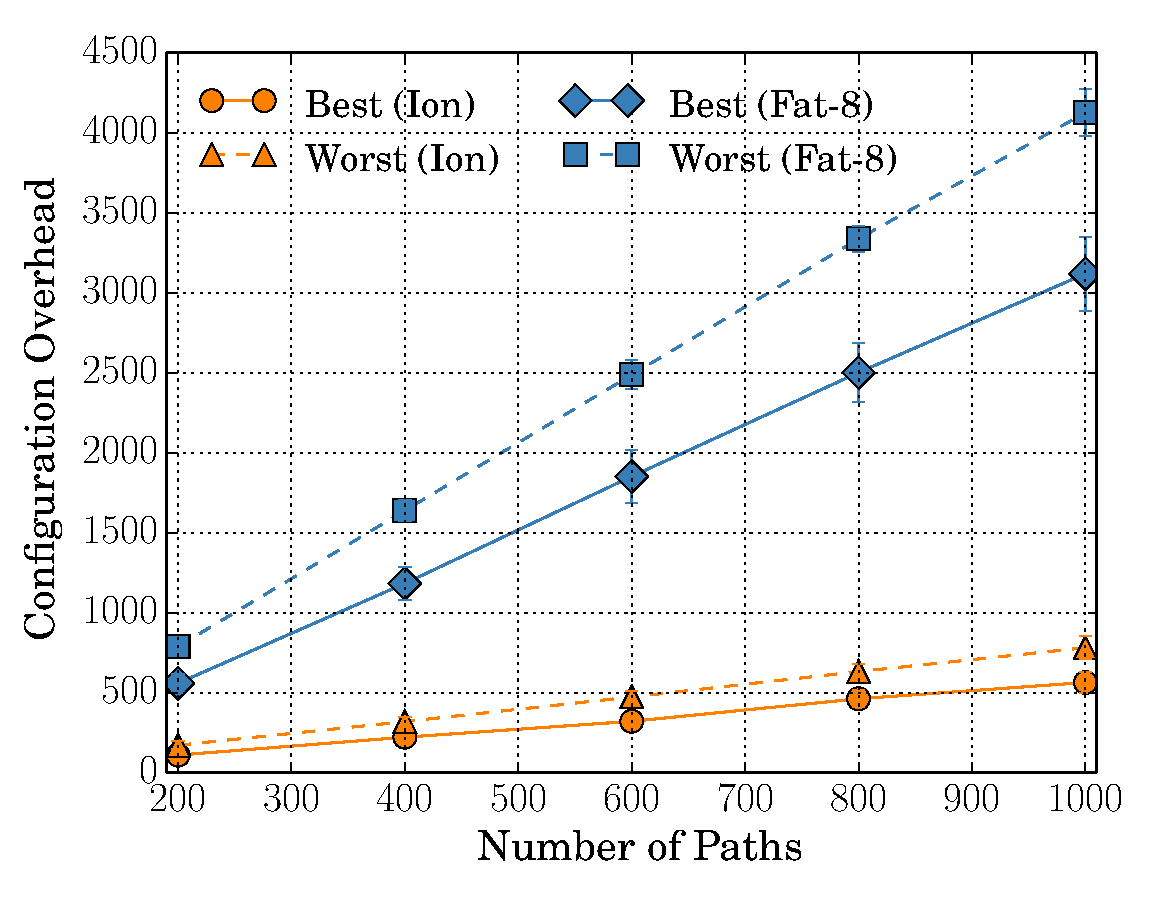
\includegraphics[width=0.7\columnwidth]{figures/confMCMC.eps}
	\compactcaption{MCMC Lines of Conf}
	\label{fig:confmcmc}
\end{figure}

\begin{figure}[t]
	\centering
	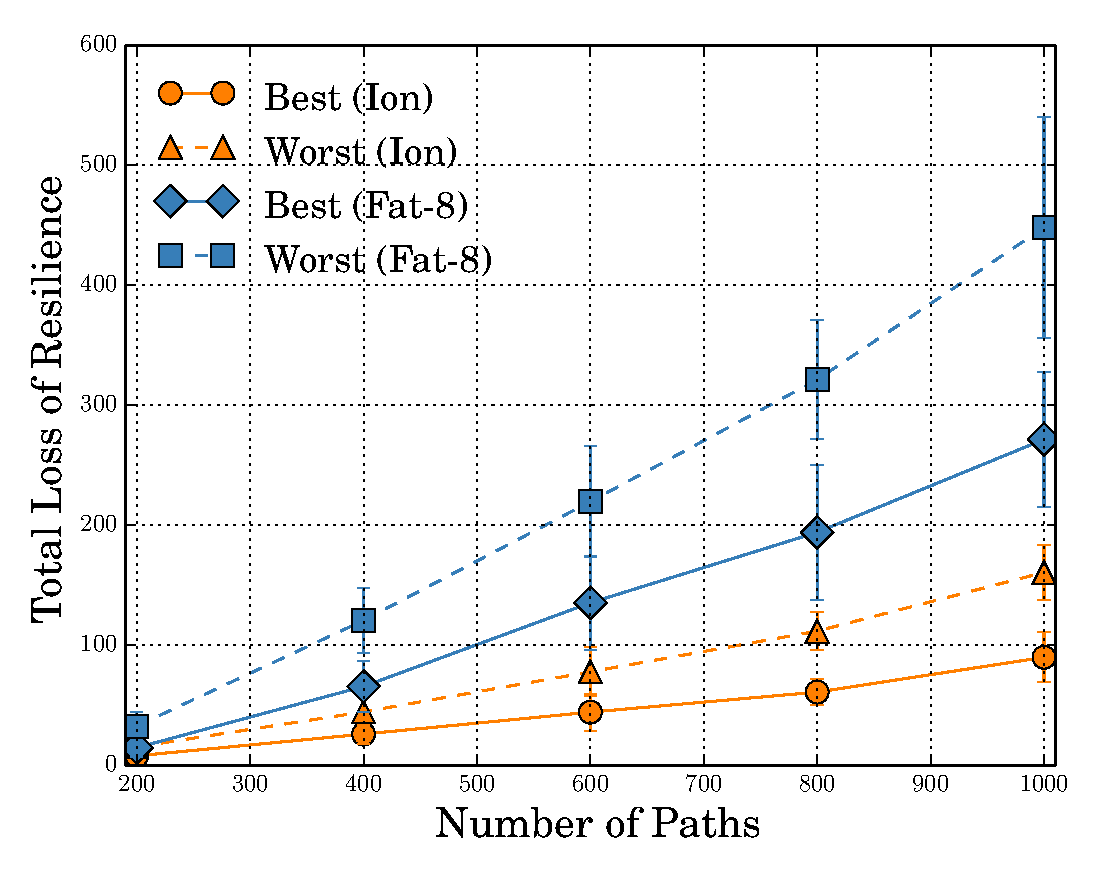
\includegraphics[width=0.7\columnwidth]{figures/TRLMCMC.eps}
	\compactcaption{MCMC TRL}
	\label{fig:trlmcmc}
\end{figure}



\section{Evaluation}
\section{Related Work}\label{sec:related}
\paragraph{Centralized control} Programming routers for centralized
control has been an active area of research in recent times. One of
the first systems, RCP~\cite{rcp}, supported logically central BGP
configuration. The more recent Fibbing~\cite{fibbing} system provides
centralized control over distributed routing by creating fake nodes
and fake links to steer the traffic in the network through paths that
are not the shortest, similar to how \name uses static routes.  Both
approaches face the issue of forwarding loops in the network during
failures. Fibbing and \name differ in the specific algorithms to solve
the synthesis problem.  \name does offer key advantages: first, by
using static routes for steering, we do not increase the traffic in
the network, unlike the fake advertisements used in Fibbing. Second,
Fibbing by design targets a single domain and does not take into account
domain decomposition and inter-domain routing. 

%However, these fake advertisements can create
%forwarding loops in the network during failures, and the centralized
%controller has to respond to failures (response to failures can
%precomputed), thus making the controller a central point of
%failure. In contrast, our approach to distributed control plane
%synthesis can provide the same expressive power as Fibbing but avoids
%any centralized component by engineering the control plane parameters
%to match the input specifications.  


\paragraph{Configuration synthesis} 
ConfigAssure~\cite{configassure}
uses a combination of logic programming and SAT solving to synthesize
network configurations for security, 
functionality, performance and
reliability requirements specified as constraints; 
but it does not
support any notion of policy- or connectivity-resilience 
or hierarchical domain splitting.  Fortz
et. al~\cite{ospf-te} tackle the problem of optimizing OSPF weights
for performing traffic engineering, but their work is tailor-made
to just this specific problem.

Propane~\cite{propane, propaneat} tackles the specific problem of
synthesizing BGP configurations for concrete and abstract topologies
to ensure network-wide objectives hold even under failures. The policy
language of Propane is suited to specify preferences on paths and
peering policies among different autonomous systems. Propane
translates policies to a graph-based intermediate representation,
which is then compiled to device-level BGP configurations. It is
unclear how to extend Propane to incorporate domains, configuration
complexity, or OSPF routing.

SyNET~\cite{synet} tackles network-wide configuration synthesis
(Definition \ref{def:policycompliance}) in an elegant manner by
modeling the behavior and interactions of the routing protocols as a
stratified Datalog program, and using SMT to synthesize the Datalog
input such that the fixed point of the Datalog program (which
represents the network's forwarding state after the protocols have
converged) satisfies certain policies or path requirements.  While
both systems can take paths as input requirements, \name uses
a two-phase approach where OSPF weights are synthesized
separately using
LP-solvers---which are faster and parallelizable---rather than directly  
solving the whole configuration synthesis problem using SMT solvers.  
Moreover, SyNET's approach
does not deal with resilience, a key aspect we tackle in this paper,
and
SyNET does not attempt to minimize the number of static routes,
which can cause undesirable behaviors like routing loops.  Finally,
SyNET supports routers that run both OSPF and BGP protocols and can be
configured with static routes, which does not fit naturally into a
hierarchical structure where some routers only run OSPF and not
BGP. In contrast, our MCMC algorithm can look for dynamic domain
assignments.

\paragraph{Policy languages} While \name uses \genesis 
to synthesize policy-compliant paths, in the future it could use
other policy language frameworks as a front-end
too; existing frameworks offer perhaps less rich policy support but better
performance. %% Other works on
%% centralized policy enforcement for SDN are Merlin~\cite{merlin} and
%% NetKAT~\cite{netkat}.
In Merlin~\cite{merlin}, data planes that adhere to policies expressed
using regular expressions are synthesized by first intersecting the
topology with the regular expressions appearing in the policies and
then encoding reachability in the intersected graph using mixed
integer linear programming (ILP).  Merlin supports min and max
bandwidth guarantees.

NetKAT~\cite{netkat} is a domain-specific language and logic for 
specifying and verifying network packet-processing functions
for SDN, based on Kleene algebra with tests (KAT). Semantically,
a NetKAT predicate and policy is a function that takes a packet
history and produces a set of (possibly empty) packet histories. 
NetKAT can be used to express certain network-wide policies like 
reachability, waypoints using regular expressions for describing the paths, 
and programs on virtual topologies; it uses
BDDs and symbolic automata to translate global programs to local
switch programs~\cite{netkatcompiler}.
Both Merlin and NetKAT  do not support link-isolation 
to produce edge-disjoint paths, which is needed for  
our waypoint-compliance algorithm presented in Section~\ref{sec:waypointres}.
As future work, we will consider 
how to apply these other front-ends to \name.

%% However, the NetKAT semantics
%% cannot be used to express policies based on hyperproperties
%% ~\cite{hyperproperties}, i.e., 
%% the packet processing function requires multiple packet histories
%% as input. Traffic engineering or isolated paths are policies
%% based on hyperproperties.

%% While Genesis supports richer policies, its SMT-based approach is slower in synthesis. As part of future work, we will consider how

%Fine-grained traffic engineering based on online demand/flow size estimation and 
%rapid rerouting is also crucial for datacenter workloads, and extending \name's
%TE policies to fine-grained timescales is subject of future work.
%Also, the performance
%of SMT solvers with optimization objectives is quite slow, and calls for 
%domain-specific techniques to speed up the synthesis. Also, datacenter
%networks are highly symmetrical, and this symmetry can be leveraged
%to speed up synthesis (similar to the work of Plotkin et. al~\cite{symmetry} to
%speed up network verification using symmetry). The main challenges of
%using symmetry in synthesis is considering two aspects of symmetry: network
%symmetry and policy symmetry. Also, our treatment of resilience synthesis
%is preliminary and future work will be geared towards synthesizing resilient
%forwarding planes incorporating capacity constraints and traffic engineering.
 

%!TEX root = paper.tex
\section{Conclusion}
We presented \name, a system for automatically synthesizing 
highly-resilient distributed hierarchical control planes---i.e., OSPF and 
BGP router configurations---from
high-level policies. For hierarchical control planes, 
we devised algorithms based on our OSPF-BGP interaction model. In 
practice, there exists hierarchical models, we can integrate these routing
models into \name's modular two-phase approach.
Similarly, we can modify OSPF synthesis to incorporate multi-path routing
for load-balancing etc. Finally, resilience is an important requirement, 
and extending \name to support other notions of policy-resilience
for $k > 1$ link failures is subject for future work.
\section*{Acknowledgments}
We thank the anonymous reviewers and our shepherd Brighten Godfrey, 
Aaron Gember-Jacobson, 
Raajay Viswanathan, and Shuchi Chawla 
for their insightful feedback and suggestions. 
Kausik, Loris and Aditya  
are supported by the Wisconsin Institute
on Software-defined Datacenters of Madison and 
grants from Google and National
Science Foundation (CCF-1637516, CNS-1302041, CNS-1330308, CNS-1345249).

\bibliographystyle{ACM-Reference-Format}
\bibliography{references}

\appendix
\section{Proofs}
\begin{theorem}[Hardness of synthesis]
\label{thm:ospfsynth}
Given a
network with a single domain,
and a positive number $C_{sc}$,
the problem generating
a path-compliant configuration with at most $C_{sc}$ static routes
is NP-complete.
\end{theorem}
\begin{proof}
We show that the decision version of the minimum 
vertex cover problem, i.e., there exists a vertex cover
of size $ \leq k$, which is NP-complete, 
reduces to finding a set of route filters of size $ \leq k$ \
and OSPF weights for a network with only one domain. 
The latter is also in NP, so after the reduction we 
can conclude that it is also NP-complete.

Let $G = (V,E)$ be an instance of the 
minimum vertex cover problem. A set of
vertices $VC \subseteq V$ is the vertex cover
if $\forall (v_1, v_2) \in E. ~v_1 \in VC \vee v_2 \in VC$. 

We now show how to construct a topology $T=(S,L)$ 
and a corresponding set of paths $P$ that can be 
induced by route filter set $R$ such that $|R| \leq k$  
iff the corresponding $VC(R)$ is a vertex cover of 
the graph $G$ and $|VC(R)| \leq k$.

For every vertex $v \in V$: add two vertices $r_v^1$ 
and $r_v^2$ to $S$ and a directed link $r_v^1 \rightarrow r_v^2$ to $L$. 
We also assign a destination host $d_v$ for each vertex $v$. 

For every edge $(u,v) \in E$: add two vertices $s_{uv}$
and $t_{uv}$ to $S$. Add edges
connecting $s_{uv} \rightarrow s_{u}^1$, $s_{uv} \rightarrow s_{v}^1$,
$s_{u}^2 \rightarrow t_{uv}$ and $s_{v}^2 \rightarrow t_{uv}$. \Cref{fig:rfcomplexity} illustrates this construction.
\begin{figure}[H]
	\centering
	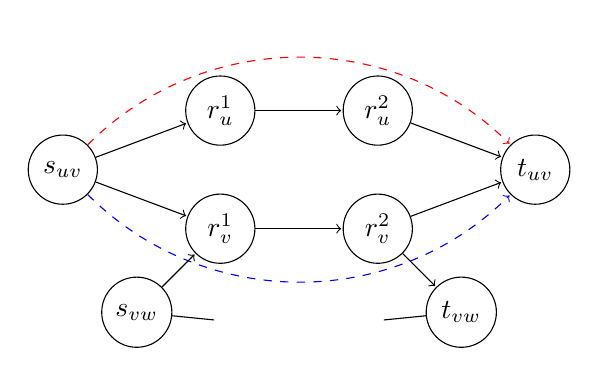
\begin{tikzpicture}[shorten >=0.5pt,node distance=1.5cm,on grid,auto,
	square/.style={regular polygon,regular polygon sides=4}] 
	\node[state] at (0,0) (s)  {$s_{uv}$}; 
	\node[state] at (2,-0.75) (v1)  {$r_v^1$}; 
	\node[state] at (4,-0.75) (v2)  {$r_v^2$};
	\node[state] at (2,0.75) (u1)  {$r_u^1$}; 
	\node[state] at (4,0.75) (u2)  {$r_u^2$}; 
	\node[state] at (6,0) (t) {$t_{uv}$};
	\node[state] (s1) [below left=of v1] {$s_{vw}$}; 	
	\node[state] (t1) [below right=of v2] {$t_{vw}$}; 	
	\path[->] 
	(s) edge  node {} (v1)
	edge  node {} (u1)
	edge [blue, dashed, bend right=45] node {} (t)
	edge [red, dashed, bend left=45] node {} (t)
	(u1) edge node {} (u2)
	(u2) edge node {} (t)
	(v1) edge node {} (v2)
	(v2) edge node {} (t)
	edge node {} (t1)
	(s1) edge node {} (v1);
	\path[-] (s1) edge node[above] {} +(1,-0.1);
	\path[-] (t1) edge node[above] {} +(-1,-0.1);
	\end{tikzpicture}
	\caption{Construction}
	\label{fig:rfcomplexity}
\end{figure}
If there was another edge $(v,w) \in E$, then
$s_{vw}$ has an edge connecting to $r_v^1$ and
$r_v^2$ has an edge connecting to $t_{vw}$ (shown
in \Cref{fig:rfcomplexity}). $s_{vw}$ will also 
have an edge to $s_w^1$ and similarily from $s_w^2$ to $t_{uw}$
as per the construction outlined above.

For each edge $(u,v) \in E$, we add two paths in $P$: 
$s_{uv} \rightarrow r_u^1 \rightarrow r_u^2 \rightarrow t_{uv}$
for destination host $d_v$ and 
$~s_{uv} \rightarrow r_v^1 \rightarrow r_v^2 \rightarrow t_{uv}$ 
for destination host $d_u$.
(dashed paths in \Cref{fig:rfcomplexity}). 

We now prove that if there exists a set of route filters
$R$ such that $|R| \leq k$ such that the resulting configurations
forwards traffic along $P$, then there exists a vertex cover $VC$
of $G$ such that $|VC| \leq k$. 

For each route filter $r \in R$, one of its endpoints 
has to be either $r_v^1$ or $r_v^2$, corresponding
to some vertex $v \in V$ (structure of topology $T$). 
We construct a set $VC(R)$ by adding the vertex $v$ 
based on the endpoints of each route filter $r \in R$.
To show that $VC(R)$ is a vertex cover of $G$, we first
prove \Cref{lemma:diamond}.

\begin{lemma} \label{lemma:diamond}
	 For each diamond formed by the input paths, atleast 1 
	 route filter on one of the edges of the paths of the diamond 
	 is required to find a valid solution to the
	 OSPF edge weights.  
\end{lemma}

\begin{proof}
Consider the following diamond % in \Cref{fig:diamond}
constructed by paths $p_1$: $s \rightarrow r_1 \rightarrow t$ 
for destination $d_1$ and $p_2$:$s \rightarrow r_2 \rightarrow t$ 
for destination $d_2$. Let us assume there exists a solution 
for the OSPF edge weights without any route filters. 

As we will describe in \Cref{sec:intra-synthesis}, 
to ensure $p_1$ is the shortest path from $s$ to $t$, the following
linear inequality is added to ensure $p_1$ is shorter than the
path from $s$ to $t$ via $r_2$: 
\begin{equation} \label{eq:diamond1}
	e(s,r_1) + e(r_1, t) < e(s, r_2) + e(r_2,t)
\end{equation}
$e(s,r_1)$ denotes the weight of edge $s \rightarrow r_1$.
Since $p_2$ is also the shortest path from $s$ 
to $t$, the linear inequality added is:
\begin{equation}  \label{eq:diamond2}
e(s,r_2) + e(r_2, t) < e(s, r_1) + e(r_1,t)
\end{equation}
Since there are no route filters on the edges
of $p_1$ and $p_2$, none of the above equations are 
eliminated (\Cref{sec:routefilter}). 
Adding equations \ref{eq:diamond1} and  \ref{eq:diamond2} 
yields the inequality $0 < 0$, which is inconsistent 
and therefore, no solution to 
the edge weights exists for this system of equations, 
which contradicts our assumption. Therefore,
for each diamond formed by the input paths, atleast 1 
route filter on one of the edges of the paths of the diamond 
is required to find a valid solution to the
OSPF edge weights.  
\end{proof}

For every edge $(u,v) \in E$, the constructed paths from 
$s_{uv}$ to $t_{uv}$ form a diamond. Thus, by lemma 1, 
the diamond corresponding to each edge in $G$ 
requires atleast one route filter to eliminate
the inconsistency caused by the diamond, thus, one 
of vertices $\{u,v\}$ will be in $VC(R)$, and edge $(u,v)$
is covered. Thus, if $R$ eliminates all diamond inconsistencies
to find a solution to the OSPF weights, the corresponding set
$VC(R)$ covers all edges in $E$. Therefore, $VC(R)$ is a vertex
cover. 

Thus, by finding a set of route filters $R$ such that $|R| \leq k$
such that all the diamond inconsistencies are eliminated, and there
exists OSPF weights $W$ such that the configurations forward traffic
along $P$, we can find a vertex cover $VC$ for graph $G$ such that
$|VC| \leq k$. 

This transformation is polynomial, the constructed 
network topology $T$ has $2|V| + 2|E|$ nodes, 
$|V| + 4|E|$ links and $2|E|$ paths. Therefore, OSPF
configuration synthesis with number of route filters $\leq k$ is
NP-complete. Thus, OSPF synthesis with minimal number of 
route filters is NP-hard. 
\end{proof}



%% Appendix

\end{document}
